% ****** Start of file apssamp.tex ******
%
%   This file is part of the APS files in the REVTeX 4.2 distribution.
%   Version 4.2a of REVTeX, December 2014
%
%   Copyright (c) 2014 The American Physical Society.
%
%   See the REVTeX 4 README file for restrictions and more information.
%
% TeX'ing this file requires that you have AMS-LaTeX 2.0 installed
% as well as the rest of the prerequisites for REVTeX 4.2
%
% See the REVTeX 4 README file
% It also requires running BibTeX. The commands are as follows:
%
%  1)  latex apssamp.tex
%  2)  bibtex apssamp
%  3)  latex apssamp.tex
%  4)  latex apssamp.tex
%
\documentclass[%
reprint,
%superscriptaddress,
%groupedaddress,
%unsortedaddress,
%runinaddress,
%frontmatterverbose, 
%preprint,
%preprintnumbers,
%nofootinbib,
%nobibnotes,
%bibnotes,
amsmath,amssymb,
aps,
pra,
%prb,
%rmp,
%prstab,
%prstper,
floatfix,
]{revtex4-2}

\usepackage{subfiles}
\usepackage{graphicx}% Include figure files
\usepackage{dcolumn}% Align table columns on decimal point
\usepackage{bm}% bold math
\usepackage{float}
\usepackage{mathtools}
\usepackage{xcolor}
\usepackage{physics}
\usepackage{dsfont}
\usepackage{tcolorbox}
\usepackage{float}
\usepackage{tensor}
\usepackage{hyperref}% add hypertext capabilities
%\usepackage[mathlines]{lineno}% Enable numbering of text and display math
%\linenumbers\relax % Commence numbering lines

%\usepackage[showframe,%Uncomment any one of the following lines to test 
%%scale=0.7, marginratio={1:1, 2:3}, ignoreall,% default settings
%%text={7in,10in},centering,
%%margin=1.5in,
%%total={6.5in,8.75in}, top=1.2in, left=0.9in, includefoot,
%%height=10in,a5paper,hmargin={3cm,0.8in},
%]{geometry}
\newcommand{\Hp}{\mathcal{H}}
\renewcommand{\thesection}{\arabic{section}}
\renewcommand{\thesubsection}{\thesection.\arabic{subsection}}
\renewcommand{\thesubsubsection}{\thesubsection.\arabic{subsubsection}}
\renewcommand{\figurename}{Fig.}
\renewcommand{\tablename}{Table}
\makeatletter
\renewcommand{\subsubsection}{%
	\@startsection
	{subsubsection}%
	{3}%
	{\z@}%
	{.8cm \@plus1ex \@minus .2ex}%
	{.5cm}%
	{\normalfont\small\centering}%
}
\makeatother
\renewcommand{\L}{\mathcal{L}}
\renewcommand{\O}{\mathcal{O}}
\newcommand{\f}[2]{\frac{#1}{#2}}
\newcommand{\p}{\partial}
\makeatletter
\renewcommand{\p@subsection}{}
\renewcommand{\p@subsubsection}{}
\makeatletter

\begin{document}
	
\title{Application of Regression and Resampling on USGS Terrain Data}
\author{Isak O. Rukan}
\email{icrukan@uio.no}
\author{Edvard B. Rørnes}
\email{e.b.rornes@fys.uio.no}
\affiliation{Institute of Physics, University of Oslo,\\0371 Oslo,  Norway}
\date{\today}

\begin{abstract}
	Regression models are widely used for analyzing and predicting data in many fields. We investigate and compare three regression models\footnote{\href{https://github.com/EdvardRornes/FYS-STK4155/tree/main/Project1}{Github}}: Ordinary Least Squares, Ridge, and Least Absolute Shrinkage and Selection Operator. These were applied and analyzed on a two-dimensional Franke function and later tested on real terrain data from the US Geological Survey Earth Explorer \cite{USGS_EarthExplorer}. The models' performances are evaluated using metrics such as the Mean Squared Error and the coefficient of determination $R^2$. The bias-variance trade-off for OLS is studied where it was found that the optimal polynomial degree for the Franke function was $p=4$. We used resampling techniques such as bootstrapping and cross-validation to probe the quality of the evaluations and determine the predictiveness and generalizability of the models. The analysis of the terrain data suggests that there is a slightly larger complexity the best fits were found around $p\sim7$. In our analysis of both the Franke function and the terrain data the best performing method was Ridge regression with OLS following shortly after. LASSO performed worse than the other regression methods by a small margin for lower polynomial degrees, likely stemming from the polynomial coefficients not following a Laplace distribution.
\end{abstract}

\maketitle

\section{Introduction}
Regression models are essential tools in data analysis and prediction, particularly within the realm of physics. They are used to enable understanding of the relationships between different variables and improve our ability to create predictions. In this report we study and compare three common regression techniques: Ordinary Least Squares (OLS), Ridge and Least Absolute Shrinkage and Selection Operator (LASSO) regression. Each come with their unique strengths and weaknesses that make them suitable for different data sets. 

OLS is the simplest and most foundational method which estimates relationship by minimizing the difference between observed and predicted values. A large downside with OLS is when there are many related variables as this can lead to unstable coefficient estimates \cite{Bishop2006}. Ridge regression can partially fix this issue by adding a penalty to large coefficients via a regulator $\lambda$, effectively allowing us to shrink the coefficients with a new input parameter. This in turn creates a more stable model in the event of correlated variables. LASSO regression takes this a step further by once again shrinking coefficients, but also setting some of them to zero \cite{hastie01statisticallearning}. This allows LASSO to effectively choose important variables, which may be helpful when pursuing a simpler model.

To compare these regression methods, we use a two-dimensional Franke function which allows us to test the performance of each under controlled conditions. Later we apply each method to real terrain data which is obtained from \cite{USGS_EarthExplorer}.

The regression methods are evaluated by considering their Mean Squared Error (MSE) and coefficient of determination $R^2$. Further to make our evaluation more reliable, resampling techniques such as bootstrapping and cross-validation are used. These methods provide a quantitative description of how well each model performs on different data sets.
\section{Theory}
All claims made in this section which require relatively lengthy derivations are derived in Appendix \ref{Appendix:Derivations}. The general structure of all our models is that we have some data set $\{x_i,y_i\}$ where $i\in\{0,1...,n-1\}$ where $x_i$ are independent variables whilst $y_i$ are dependent variables. The data is assumed to be described by
\begin{align}
	\bm y=f(\bm x)+\bm \varepsilon,
	\label{eq:data}
\end{align}
where $f$ is some continuous function which takes $\bm x$ as input and $\bm\varepsilon$ is a normal distributed error $\bm\varepsilon\sim\mathcal{N}(0,\sigma^2)$. The function $f$ will then be approximated with a model $\tilde{\bm y}$ in which we will consider a polynomial expansion with coefficients $\beta_i$ up to degree $p$:
\begin{align}
	\tilde{y}_i=\sum_{j=0}^{p}\beta_j x_i^j.
	\label{eq:model}
\end{align}
Defining the $n\times p$ design matrix $\bm X$ with elements $X_{ij}=(x_i)^j$ we can rewrite this as
\begin{align}
	\tilde{\bm y}=\bm X\bm\beta.
\end{align}
Further, each model will be defined with a different cost function $C(\bm\beta)$ which we minimize to find the coefficients for each respective model.

The metrics MSE and $R^2$ which we use to analyze each method are defined by:
\begin{align}
	\text{MSE}(\bm y,\tilde{\bm{y}})&\equiv\frac{1}{n}\sum_{i=0}^{n-1}(y_i-\tilde y_i)^2,\\
	R^2&\equiv1-\frac{\sum_{i=0}^{n-1}(y_i-\tilde y_i)^2}{\sum_{i=0}^{n-1}(y_i-\bar y)^2},
\end{align}
where $\bar y\equiv\frac{1}{n}\sum_{i=0}^{n-1}y_i$ is the mean value of $\bm y$. Here we can see that if $\tilde{\bm{y}}=\bm y$ then $R^2=1$ and $\text{MSE}=0$ implies that we have perfect accuracy. Further if $\tilde{\bm{y}}$ is simply the mean then $R^2=0$ implying that our fit performs as well taking the mean. Finally if $R^2<0$ it means that our approximation is worse than simply taking the mean. Thus for a good fit we would expect a small MSE and an $R^2$ score closer to $1$.

\subsection{OLS}
\label{sec:THEORY_OLS}
OLS is a primitive method used in linear regression to estimate coefficients of a linear model. The cost function in OLS is simply defined as the MSE:
\begin{align}
	C_\text{OLS}(\bm\beta)=\f1n(\bm y-\tilde{\bm y})^2.
	\label{eq:cost_ols}
\end{align}
As mentioned prior, the coefficients $\bm\beta$ are found by minimizing the cost function, i.e. taking the derivative w.r.t. $\bm\beta$. This results in
\begin{align}
	\bm\beta_\text{OLS}=(\bm X^T\bm X)^{-1}\bm X^T\bm y,
	\label{eq:beta_ols}
\end{align}
which yields the model
\begin{align}
	\tilde{\bm y}_\text{OLS}=\bm X\bm \beta_\text{OLS}.
\end{align}
Assuming our data takes the form of (\ref{eq:data}) then the expectation value $\bm y$ is
\begin{align*}
	\mathbb{E}(y_i)=\mathbb{E}(f(x_i))=X_{ij}\beta_j\equiv\bm X_{i,*}\bm\beta,
\end{align*}
since $\mathbb{E}(\varepsilon_i)=0$ follows from its definition. The variance of $\bm y$ is given by
\begin{align*}
	\text{Var}(y_i)=\text{Var}(\varepsilon_i^2)=\sigma^2,
\end{align*}
which yields $y_i\sim\mathcal{N}(\bm X_{i,*}\bm\beta,\sigma^2)$. The expectation value of the optimal parameters $\hat{\bm\beta}$ can be found to be
\begin{align*}
	\mathbb{E}(\hat{\bm\beta}_\text{OLS})=\bm\beta,
\end{align*}
with the variance
\begin{align*}
	\text{Var}(\hat{\bm\beta}_\text{OLS})=\sigma^2(\bm X^T \bm X)^{-1}.
\end{align*}

\subsection{Ridge}	\label{sec:THEORY_Ridge}
Ridge regression is an extension of OLS where define the cost function as a modified version of the OLS cost function with an added penalty term which is proportional to the coefficients $\beta_i^2$:
\begin{align}
	C_\text{Ridge}(\bm\beta)=C_\text{OLS}(\bm\beta)+\lambda\bm\beta^2.
	\label{eq:cost_ridge}
\end{align}
Here $\lambda\geq0$ is a regularization parameter, or commonly referred to as a hyperparameter, which controls the strength of this additional penalty. This regulator essentially drives the magnitude of these coefficients allowing for more tweaking in the parameter space. This parametrization of course includes the constraint that $\bm{\beta}^2\leq t$ for some $t<\infty$ such that we can choose our arbitrary parameter $\lambda\geq0$ to be sufficiently small s.t. the cost function (\ref{eq:cost_ridge}) does not diverge. The optimal parameters for Ridge regressions can again be found by the same process as for OLS:
\begin{align}
	\bm{\beta}&=(\bm{X}^T\bm{X}+\lambda\bm{I})^{-1}\bm{X}^T\bm{y}.
	\label{eq:beta_ridge}
\end{align}
Here we can see that the effect of adding this penalty term is essentially taking $(\bm X^T\bm X)^{-1}\to(\bm X^T\bm X+\lambda\bm I)^{-1}$ when compared to the OLS case. In the past this was generally the starting point for Ridge regression in the cases where the matrix $\bm X^T\bm X$ was not invertible. A direct way of seeing the effect of the regulator is by considering the singular value decomposition (SVD) of $\bm X$. Doing so one can show that 
\begin{align}
	\tilde{\bm{y}}_\text{Ridge}=\sum_{j=0}^{p-1}\bm{u}_j\bm{u}_j^T\frac{\sigma_j^2}{\sigma_j^2+\lambda}\bm{y},
	\label{eq:svd_ridge}
\end{align}
where $\bm u_i$ is the $i$-th row of the orthogonal matrix $\bm U$ stemming from the SVD: $\bm X=\bm U\bm \Sigma\bm V$. Since $\lambda\geq0$ then this added factor compared to OLS is $\leq1$. We can then see that Ridge regression effectively suppresses all the coefficients, thus $\lambda$ is often called the ``shrinkage" factor. 

\subsection{LASSO}	\label{sec:THEORY_LASSO}
Similarly to Ridge, LASSO also includes a penalty factor. The cost function in this case is instead defined to be
\begin{align}
	C_\text{LASSO}(\bm\beta)=C_\text{OLS}(\bm\beta)+\lambda||\bm\beta||_1,
	\label{eq:cost_lasso}
\end{align}
where
\begin{align*}
	||\bm\beta||_k\equiv\left[\sum_{i=0}^{n-1}|\beta_i|^k\right]^{1/k}
\end{align*}
is the $L^k$ norm of $\bm\beta$. Taking the derivative of (\ref{eq:cost_ridge}) w.r.t. $\bm \beta$ and requiring that this becomes zero we have
\begin{align}
	0=\pdv{C_\text{LASSO}}{\bm\beta}=-2\bm X^T(\bm y-\bm X\bm\beta)+\lambda\,\text{sgn}(\bm\beta).
\end{align}
This has the added benefit of being able to set certain parameters to be $0$ instead of suppressing them, at the cost of losing analytical expressions for $\bm\beta$ in non-trivial cases.

\subsection{Connection to Statistics}
\label{sec:stats}
The three aforementioned regression techniques all have relatively simple connections to statistical probability distribution functions. Assuming that the likelihood of an event $y_i$ with the input variables $\bm X$ and parameters $\bm\beta$ is given by a Gaussian distribution:
\begin{align}
	p(y_i,\bm X|\bm\beta)=\prod_{i=0}^{n-1}\frac{1}{\sqrt{2\pi\sigma^2}}\exp\left[-\frac{(y_i-\bm X_{i,*}\bm\beta)^2}{2\sigma^2}\right].
\end{align}
Further assuming that all events are independent and identically distributed the total probability density function takes the form
\begin{align}
	p(\bm y,\bm X|\bm\beta)=\prod_{i=0}^{n-1}p(y_i,\bm X|\bm\beta),
\end{align}
then taking the negative logarithm of the above and defining that as our cost function we can arrive at the exact expression for the cost function that we defined earlier in \eqref{eq:cost_ols}. A similar analysis for Ridge can be done. Using Bayes' theorem we have that $p(\bm\beta|\bm X,\bm y)\propto p(\bm y,\bm X|\bm\beta)p(\bm\beta)$ we then feed in the prior:
\begin{align}
	p(\beta_i)=\exp\left[-\frac{\beta_i^2}{2\tau^2}\right],
\end{align}
one arrives at the probability of the coefficients $\bm\beta$ given the data $\bm y$
\begin{align}
	p(\bm\beta|\bm X,\bm y)\propto p(\bm y,\bm X|\bm\beta)\cdot\prod_{i=0}^{p-1}\exp\left[-\frac{\beta_i^2}{2\tau^2}\right].
\end{align}
Again, defining the cost function as the negative logarithm of this expression one arrives at the Ridge cost function with $\lambda=1/(2\tau^2)$. Finally for LASSO one assumes that the initial probability is given by the same as OLS but with the addition of the $\beta$ coefficients following a Laplace distribution
\begin{align}
	p(\beta_i)=\exp\left[-\frac{|\beta_i|}{\tau}\right],
\end{align}
one arrives at the LASSO cost function with $\lambda=1/\tau$. 

These statistical connections help us better understand the assumptions made with each technique. OLS implicitly assumes that each event $y_i$ are all independent and Gaussian. When this is not the case one should not be surprised if OLS performs poorly. Ridge and LASSO however do account for the chance that there are correlated events, and assumes that the coefficients we compute are themselves Gaussian or Laplace distributed respectively. The hyperparameter $\lambda$ now has a clear interpretation, i.e. that we essentially insert a standard deviation of the $\beta$ coefficients. The performance of these latter two can then also be used to indicate which distribution more accurately describes the coefficients.

\subsection{Bias-Variance}
The so-called Bias-Variance Trade-Off can be summarized in a single equation:
\begin{align}
	\mathbb{E}[(\bm y-\tilde{\bm y})^2]=\text{Bias}[\tilde{\bm y}]+\text{Var}[\tilde{\bm y}]+\sigma^2,
	\label{eq:MSE-bias-var}
\end{align}
where the bias is defined as $\mathbb E[(f(\bm x)-\mathbb E[\tilde{\bm y}])^2]$. The LHS of (\ref{eq:MSE-bias-var}) is the expected value of the MSE which tells us how well the model's predictions match the true data on average. The equation shows that we can decompose this expected MSE into 3 different components.
\begin{itemize}
	\item Bias: This quantity measures how much the model's average prediction differs from its true value. A high bias implies that the assumptions and simplifications which the model is built on are not valid, i.e. that we are underfitting the data.
	\item Var: The variance measures how much the model's predictions vary when trained on different datasets. It captures the sensitivity of the model to small changes in the training data. A high variance suggests overfitting, meaning it performs well on the training data but may be capturing noise or false patterns.
	\item $\sigma^2$: This is the irreducible error or noise in the data itself which cannot be explained by the model.
\end{itemize}
The idea is to minimize the LHS of (\ref{eq:MSE-bias-var}), so clearly we want to minimize both the bias and variance at the same time. However these are correlated to one another, so lowering e.g. the bias can in general increase the variance and vice-versa. So bias-variance trade-off is essentially trying to optimize the complexity of the model such that we neither overfit nor underfit the model such that it can be generalized to other cases whilst not being too simplistic. These quantities can then be used as means to fine tune a model.

\subsection{Resampling}
Resampling techniques are critical in understanding the performance and robustness of a model. They tend to better show how well a model will do on data it has not seen before, and are thus useful for diagnosing problems like over- and underfitting. In this report focus on two resampling methods: bootstrapping and cross-validation.

\subsubsection{Bootstrap} 
Bootstrapping is a statistical method that involves taking random samples with replacement from the original dataset to create several new datasets. These datasets are the same size as the original dataset, but since our sampling was done with replacement, some observations are presented more than once whilst others are eliminated. Here we train and evaluate a model over each of these resampled datasets allowing us to estimate how the performance varies across different datasets. This method is particularly important when the datasets are small as it heavily increases the amount information that can be extracted from a given data set. Averaging across all the performance metrics from the bootstrap samples can provide a clearer description of how well our model performs. 

\subsubsection{Cross-Validation} 
$k$-fold cross-validation is the other resampling method which we considered in this project. In $k$-fold cross-validation, the dataset is divided into $k$ subsets (or folds). The model is trained on $k-1$ of these folds and tested on the remaining fold. This process is repeated $k$ times, with each fold being used as the test set exactly once. The performance metrics, MSE and $R^2$, are averaged over the $k$ iterations to provide a more reliable estimate of how the model performs on unseen data.

Cross-validation is particularly advantageous for its ability to reduce the variance of performance estimates by using different portions of the data for both training and validation. In our analysis, we used 5-fold cross-validation to evaluate the stability and predictive power of each regression method. This method gave us a clearer picture of how each model generalizes, helping us tune the hyperparameters, such as the regularization parameter $\lambda$ for Ridge and LASSO.

Both resampling techniques are used to gain insight into the models performance and helps us ensure that the conclusions drawn from our analysis are not overly dependent on a particular division of the dataset.

\subsection{Scaling}
Data scaling is an important tool in machine learning and data analysis. It may be used to simply make data more understandable as to keep them on a more human friendly scale, or if the data varies over several order of magnitude can be used to avoid numerical error and instability. Two most common ways to scale data are \texttt{MIN-MAX} and \texttt{StandardScaling}. MIN-MAX does as its name suggests; the range of the feature $x_i$ gets scaled to the interval $[a,b]$ one applies the following transformation
\begin{align}
	x_i\to(b-a)\frac{x_i-\text{min}(x_i)}{\text{max}(x_i)-\text{min}(x_i)}-a.
\end{align}

StandardScaling however subtracts the mean value of the sample from each data point and divides this by the standard deviation of the sample:
\begin{align}
	x_i\to\frac{x_i-\bar x_i}{\sigma(x_i)}.
\end{align}


\section{Implementation}
In this project we look to implement the three polynomial regression methods: OLS, Ridge and  LASSO, on 2D surface functions \(f(x,y)=z\). Before testing our models on actual data, we work with the Franke function which is visualized in Fig. \ref{fig:frankefunction}. and is defined by:
\begin{align}	\label{eq:franke}
	f(x,y)&=\frac{3}{4}\exp(-\frac{(9x-2)^2}{4}-\frac{(9y-2)^2}{4})\nonumber\\
	&+\frac{3}{4}\exp(-\frac{(9x+1)^2}{49}-\frac{(9y+1)^2}{10})\nonumber\\
	&+\frac{1}{2}\exp(-\frac{(9x-7)^2}{4}-\frac{(9y-3)^2}{4})\nonumber\\
	&-\frac{1}{5}\exp(-(9x-4)^2-(9y-7)^2).
\end{align}
\begin{figure}[H]
	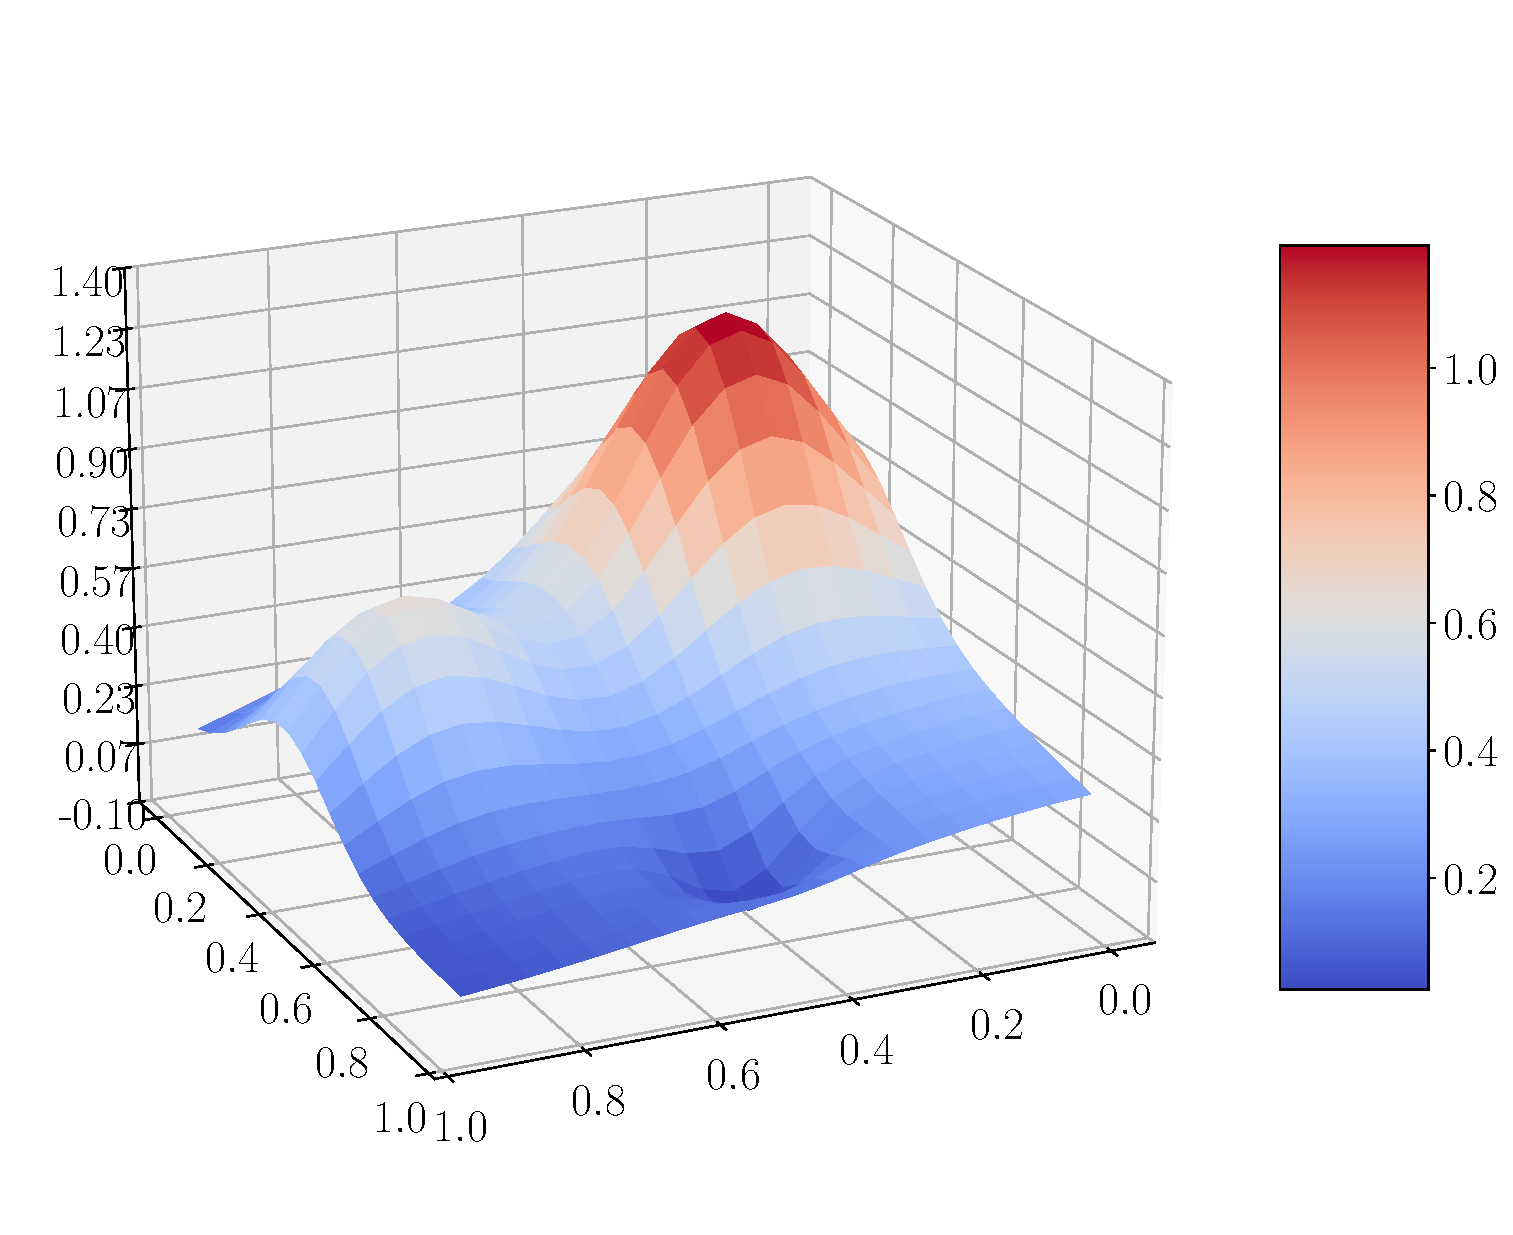
\includegraphics[width=\linewidth]{Python/Figures/FrankeFunction.pdf}
	\caption{Visualization of the Franke function (\ref{eq:franke})}
	\label{fig:frankefunction}
\end{figure}
Here we input $x,y\in[0,1]$ implying that we have already essentially scaled the data with MIN-MAX scaling. Since considering the function for negative values of $x$ and $y$ essentially gives us a different surface we have decided that there is no reason to perform StandardScaling for this case. As such we proceed without any further scaling of the data for the Franke function. 

To perform an analysis on this function we consider a polynomial fit up to degree $n$ analogous to (\ref{eq:model}) where:
\begin{align}
	\tilde{\bm{z}}&=\f1{n+1}\sum_{i=0}^{n}\bigg(\bm\beta_{0,0}\nonumber\\
	&+\bm\beta_{1,0}x_i+\bm\beta_{1,1}y_i\nonumber\\
	&+\bm\beta_{2,0}x_i^2+\bm\beta_{2,1}x_iy_i+\bm\beta_{2,2}y_i^2\nonumber\\
	&+...\nonumber\\
	&+\bm\beta_{n,0}x_i^n+\bm\beta_{n,1}x_i^{n-1}y+...+\bm\beta_{n,n-1}x_iy_i^{n-1}+\bm\beta_{n,n}y_i^n\bigg)\nonumber\\
	&=\frac{1}{n+1}\sum_{i,j=0}^{n}\sum_{\substack{k=0}}^{j}x^{j-k}_i y^{k}_i\bm\beta_{j,k}\equiv \bm X\bm\beta.
	\label{eq:bmz}
\end{align}
Here the components $x_i$ and $y_i$ are entries in the input vectors $\bm x^T=\begin{bmatrix} x_0&...&x_n \end{bmatrix}$ and $\bm y^T=\begin{bmatrix} y_0& ...&y_n \end{bmatrix}$ respectively which are our independent variables. Each $\bm\beta_{i,j}$ is a $\frac{(n+1)(n+2)}{2}$ component vector with a single non-zero entry with magnitude $|\beta_{i,j}|$ and the design matrix $\bm X$ is then an $(n+1)\times\frac{(n+1)(n+2)}{2}$ matrix of the form:
\begin{align}
	\bm X=\frac{1}{n+1}\begin{bmatrix}
		1 & x_0 & y_0 & x^2_0 & x_0y_0 & ... & x_0^n & ... & y_0^n\\
		1 & x_1 & y_1 & x_1^2 & x_1y_1 & ... & x_1^n & ... & y_1^n\\
		\vdots & \vdots & \vdots & \vdots & \vdots & \ddots & \vdots & \ddots & \vdots\\
		1 & x_n & y_n & x_n^2 & x_ny_n & ... & x_n^n & ... & y_n^n
	\end{bmatrix},
	\label{eq:design_matrix}
\end{align}
and the $\bm\beta$ vector contains the $\frac{(n+1)(n+2)}{2}$ components 
\begin{align*}
	\bm\beta^T&=\sum_{i=0}^n\sum_{j=0}^i\bm\beta_{i,j}^T=\begin{bmatrix}
		\beta_{0,0}&\beta_{1,0}&\beta_{1,1}&...&\beta_{n(n-1)}&\beta_{n,n}
	\end{bmatrix}.
\end{align*}
It should now be clear which unit vectors correspond to each term in (\ref{eq:bmz}). Note that for all practical purposes the factor $(1+n)^{-1}$ in \eqref{eq:design_matrix} can be omitted as this simply scales the $\beta_{i,j}$ coefficients with the same factor.

The inputs $\bm x$ and $\bm y$ are then split randomly into a training and test set with the latter comprising \(1/4\) of the data throughout our analysis. The general rule of thumb when allocating test data is between $1/5-1/3$ so this seemed like a reasonable middle ground. These are then used to calculate both the train and test variations of $\bm z$ and $\bm X$ using the function \href{https://scikit-learn.org/stable/modules/generated/sklearn.model_selection.train_test_split.html}{\texttt{train\_test\_split}} from \texttt{sklearn.model\_selection}. If applicable, the training and test data are then scaled after the splitting before the \(\beta\)-coefficients are calculated. The reason for doing it in this order is to avoid the test data having information such as the standard deviation of the full data to prevent data leakage.

For Ridge, \(\beta_{\text{Ridge}}\) is found by numpy's \href{https://numpy.org/doc/2.0/reference/generated/numpy.linalg.pinv.html}{\texttt{np.linalg.pinv}} to calculate the pseudoinverse of \eqref{eq:beta_ridge}. This function performs an SVD on the matrix $\bm X$ as was done in \eqref{eq:svd_ridge} to obtain an inverse even if the matrix is singular. Obtaining \(\beta_{\text{OLS}}\) is then the special case of \(\beta_{\text{Ridge}}\) with \(\lambda=0\). The \(\beta\)-coefficient for LASSO on the other hand, is computed using \href{https://scikit-learn.org/stable/modules/generated/sklearn.linear_model.Lasso.html}{\texttt{sklearn.Lasso}}. 
Sklearn's LASSO is dependent on the chosen maximum number of iterations and a tolerance parameter. Throughout this project these parameters are set to \(10^5\) and \(10^{-1}\), respectively. Lastly, the mean squared error and the $R^2$ score is then calculated using Sklearn's \href{https://scikit-learn.org/stable/modules/model_evaluation.html}{\texttt{metrics}} library.

Bootstrap was then implemented by running a for-loop over the polynomial degrees and another loop over the samples. Throughout we decided to use $x$ samples and only considered OLS for this part. The error and bias were calculated from their definitions whilst \texttt{np.var} was used to calculate the variance. Note that for the bias the approximation
\begin{align}
	\mathbb E[(f(\bm x,\bm y)-\mathbb E[\tilde{\bm{z}}])^2]\approx \mathbb E[(\bm z-\mathbb E[\tilde{\bm{z}}])^2]
\end{align}
was used. This is only valid in the low $\bm \varepsilon$ limit and thus $\bm\varepsilon=\mathcal{N}(0, 0.01)$ was used for this part.

Next $k$-fold Cross-Validation (CV) was implemented by taking in the design matrix $\bm X$, the target vector $\bm z$, the number of folds $k$ and the hyperparameter $\lambda$. The data set is then shuffled in hopes that each fold does not contain any ordering bias. The shuffled data set is split into $k$ folds where one of the folds is the test set and the remaining $k-1$ folds are used as training sets. This is iterated over $k$ times as explained in the theory section and finally the average and standard deviation over the $k$ runs are calculated.

Once everything has been implemented, we use the programs created to run on both the Franke function and the aforementioned terrain data from \cite{USGS_EarthExplorer}. For the latter we decided on two topologically interesting places: Mount Everest and the Grand Canyon. The image and contour plot for these are given in Fig. \ref{fig:GC_ME_Image_Contour}. Note however that these figures have a resolution of $2^{15}\times 2^{15}$, but for computational purposes we will limit ourselves to a small subsection of this. We implemented both MIN-MAX scaling and StandardScaling for the terrain data but opted into using StandardScaling for all the results.
\begin{figure*}
	\includegraphics[width=0.6\linewidth]{Python/Figures/Terrain/TerrainContourAndImage.pdf}
	\caption{Image and contour-plot of the Grand Canyon and Mount Everest in orange and blue respectively obtained from \cite{USGS_EarthExplorer}.}
	\label{fig:GC_ME_Image_Contour}
\end{figure*}
\newpage
\section{Results \& Discussion}

\subsection{The Franke Function}
We first consider the results obtained from the data samples generated from the Franke test function \eqref{eq:franke} using OLS, Ridge, and LASSO. In the following, unless stated otherwise, we have used $N=100$ with an added normal-distributed noise proportional to \(\varepsilon=0.1\).
\subsubsection{OLS}
%In this section we present the results of applying the OLS regression method on data generated from the Franke function in \eqref{eq:franke}. The first part of this section presents metrics and the generated \(\beta\)-coefficients using no scaling, while the last parts presents the differences of the MSE using no scaling, min-max scaling and standard scaling.

The MSE and $R^2$-score for both the train and test data as a function of the polynomial degree are given in Fig. \ref{fig:OLS_MSE_R2_degree}. The MSE of the test data exhibits a square-well shape with its lowest point at around \(p=6\), while the MSE of the training data steadily decreases as \(p\) increases. Similar traits are seen for the $R^2$ plot, however mirrored vertically. This is as expected for low $p$ as the Franke function is too complicated to be accurately described by low order polynomials. Once the polynomial degree becomes too high we start to clear signs of overfitting as we see sharp increases (decreases) in the MSE ($R^2$). 
\begin{figure}[H]
	\centering
	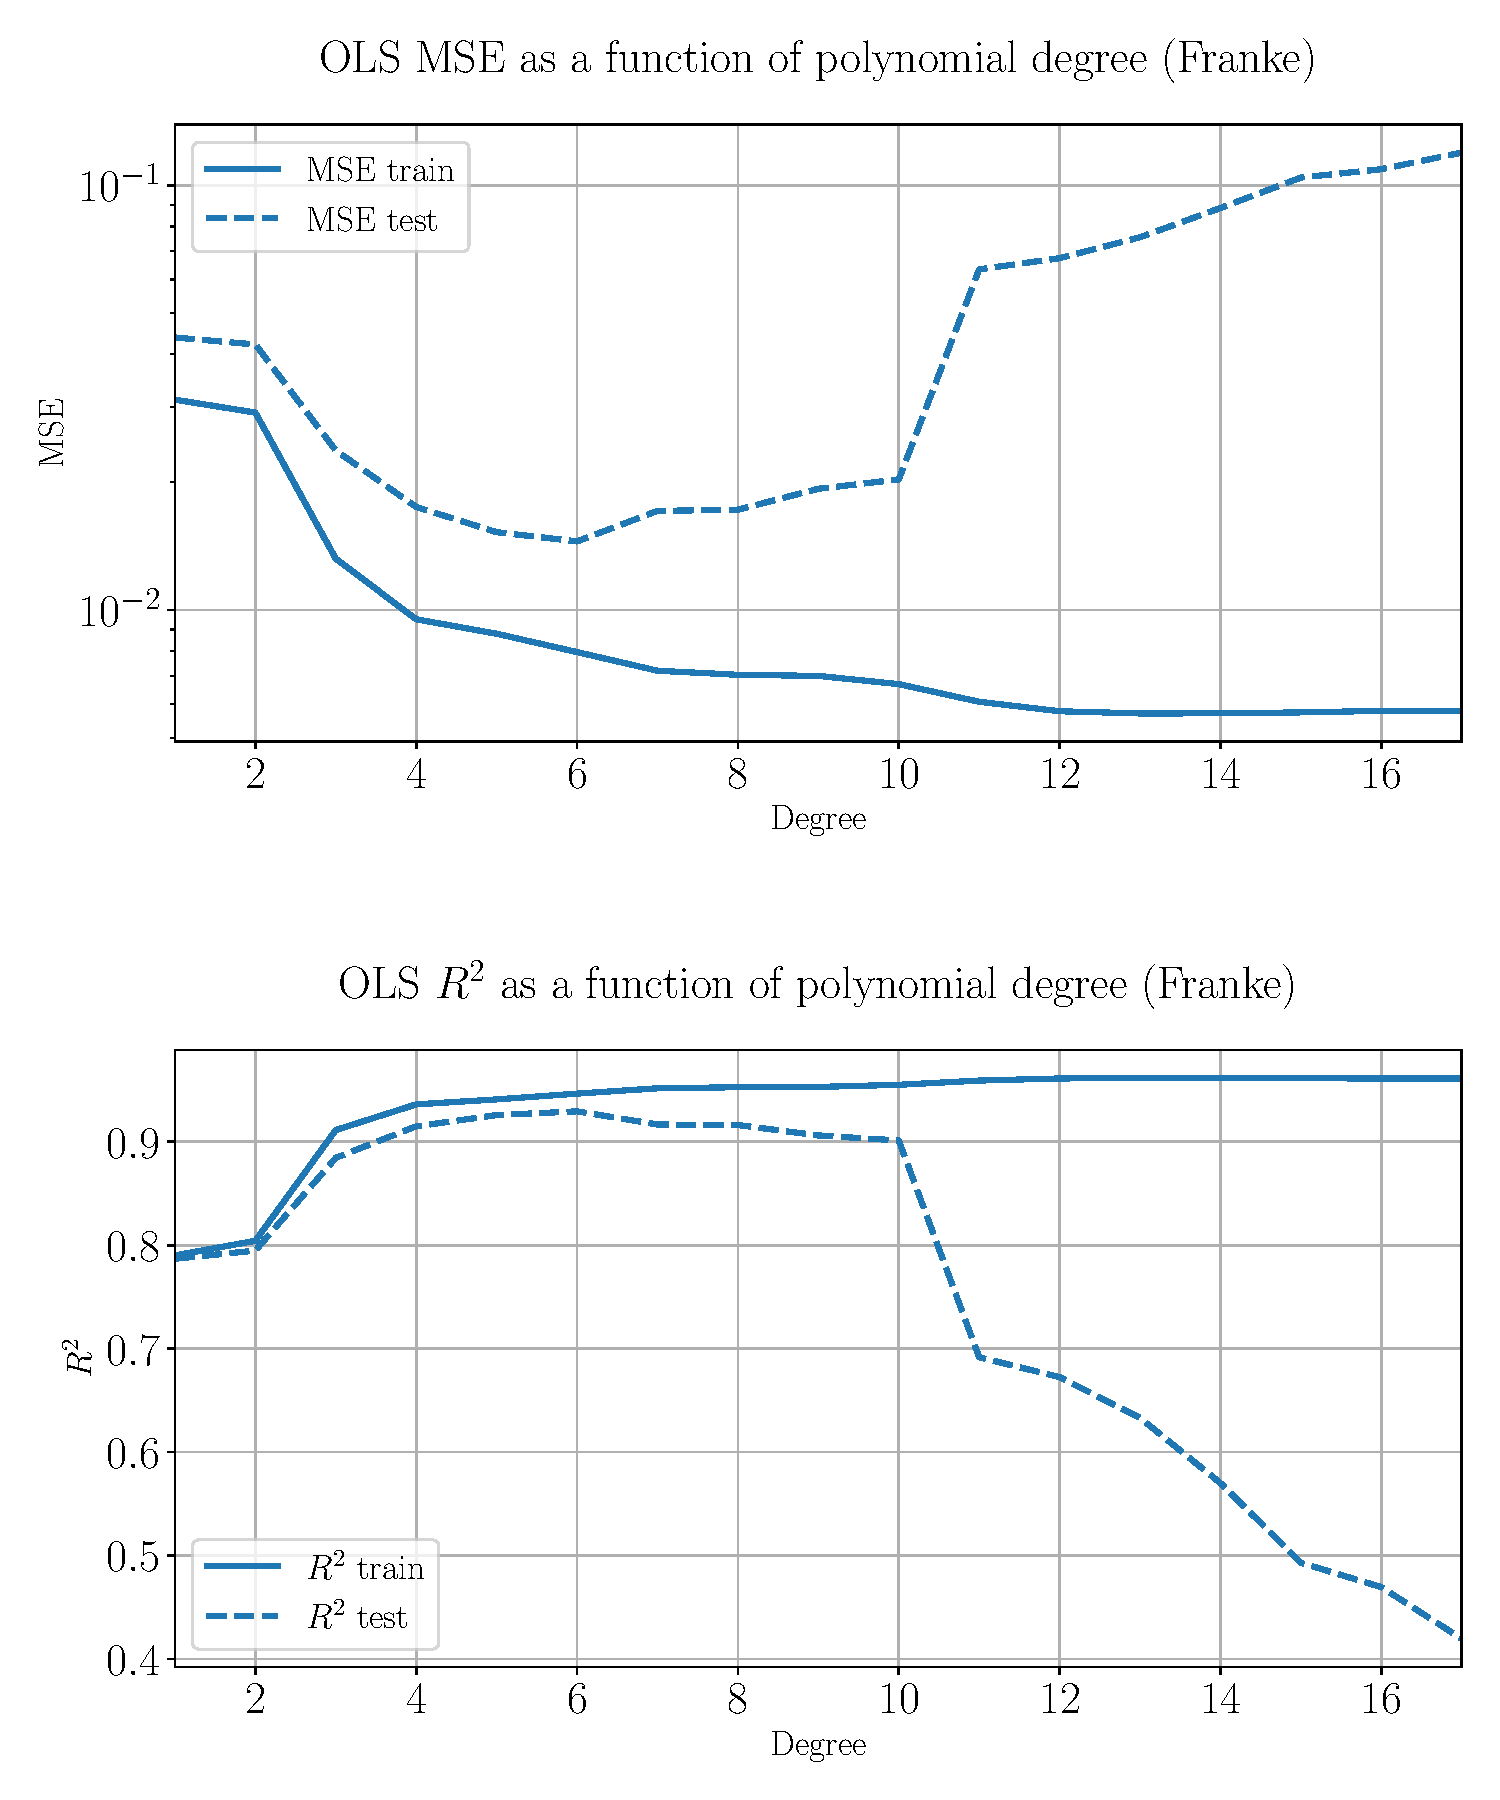
\includegraphics[width=\linewidth]{Python/Figures/OLS/OLS_MSE_R2_Unscaled.pdf}
	\caption{The MSE and $R^2$ of the train (solid) and test (dashed) data from the OLS regression method using data generated by the Franke function. The $y$-axis is logarithmic, and the $x$-axis gives the polynomial degree \(p\in[0,17]\).}
	\label{fig:OLS_MSE_R2_degree}
\end{figure}

The \(\beta\)-coefficients for \(N=100\) and \(N=1000\) datapoints can be seen in Figs. \ref{fig:OLS_beta_degree_100}. and \ref{fig:OLS_beta_degree_1000}. respectively. The color scaling indicates what polynomial degree the \(\beta\)-coefficients correspond to. For \(N=100\) the \(\beta\)-coefficients of higher degree polynomial seem larger in overal size compared to lower degree polynomial (\(p\in[0,8]\)). However, for \(N=1000\) this behavior is opposite, meaning that the \(\beta\)-coefficients for \(p\in[0,8]\) seem larger than those corresponding to higher degree polynomials.

\begin{figure}[H]
	\hspace{-7.5mm}
	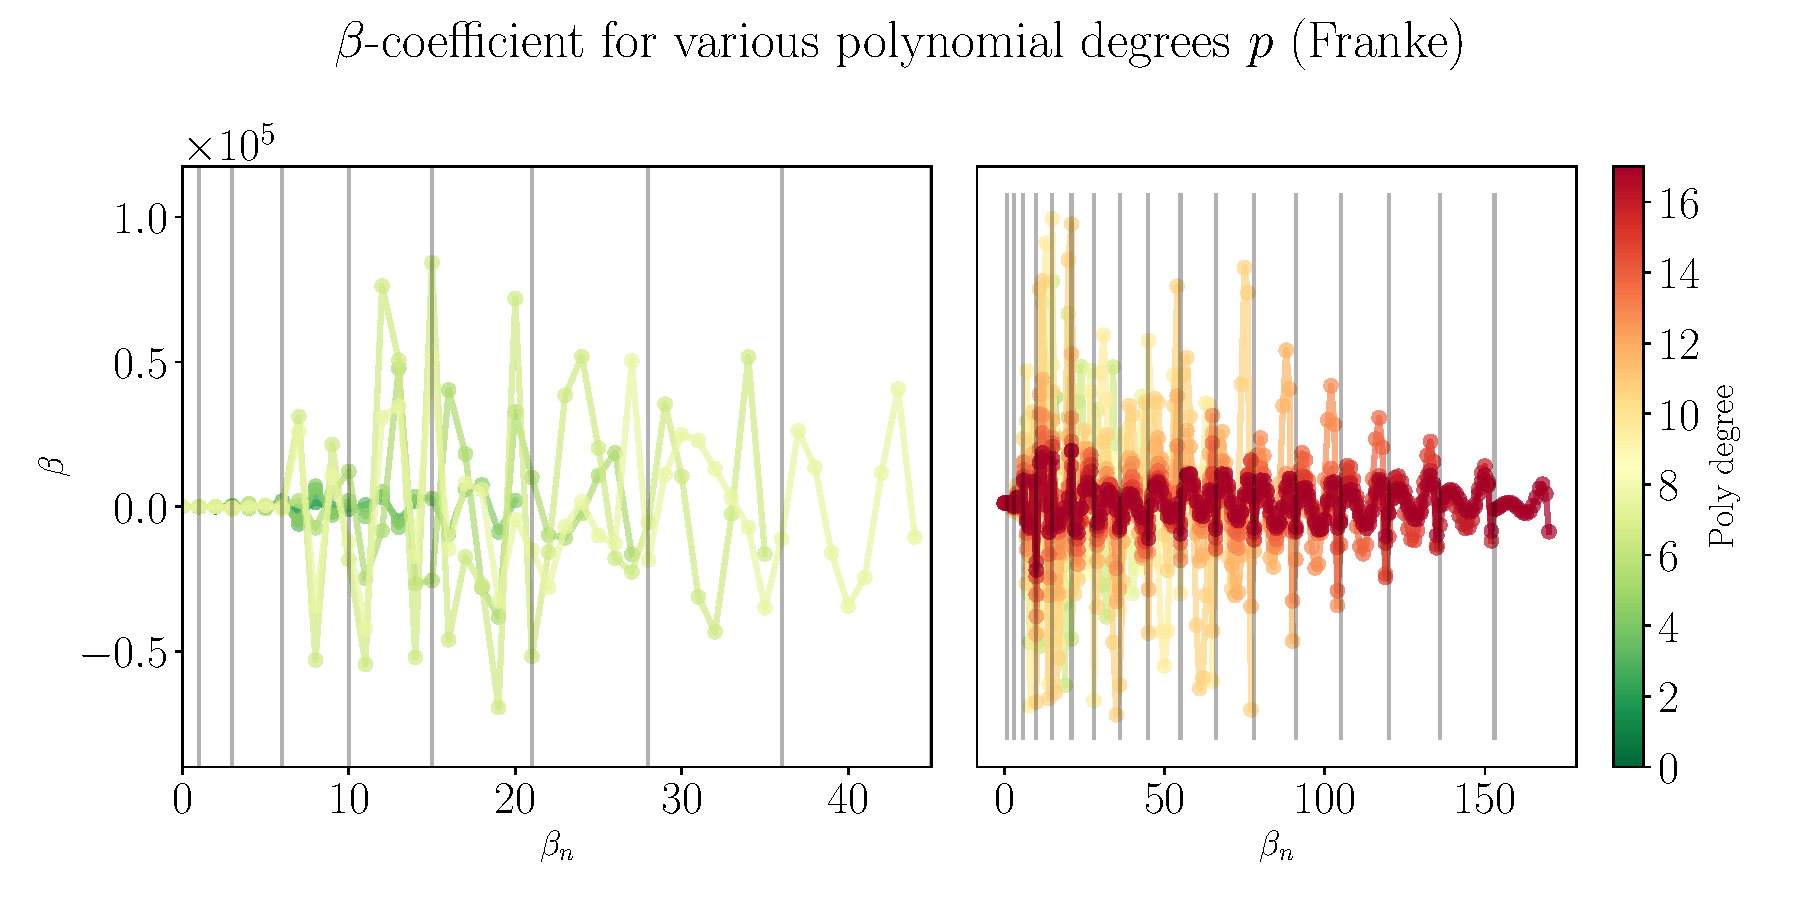
\includegraphics[width=1.15\linewidth]{Python/Figures/OLS/OLS_betano_scaling_100.pdf}
	\caption{The \(\beta\)-coefficients for the OLS-fit of \(N=100\) datapoints generated from the Franke function. The plots shows the polynomial degree from 0 (green) to 17 (red). The left hand side is restricted to \(\beta\)-coefficients corresponding to up to \(p=8\). The solid lines in the background indicate where the last coefficient of a given polynomial degree is placed.}
	\label{fig:OLS_beta_degree_100}
\end{figure}
\begin{figure}[H]
	\hspace{-7.5mm}
	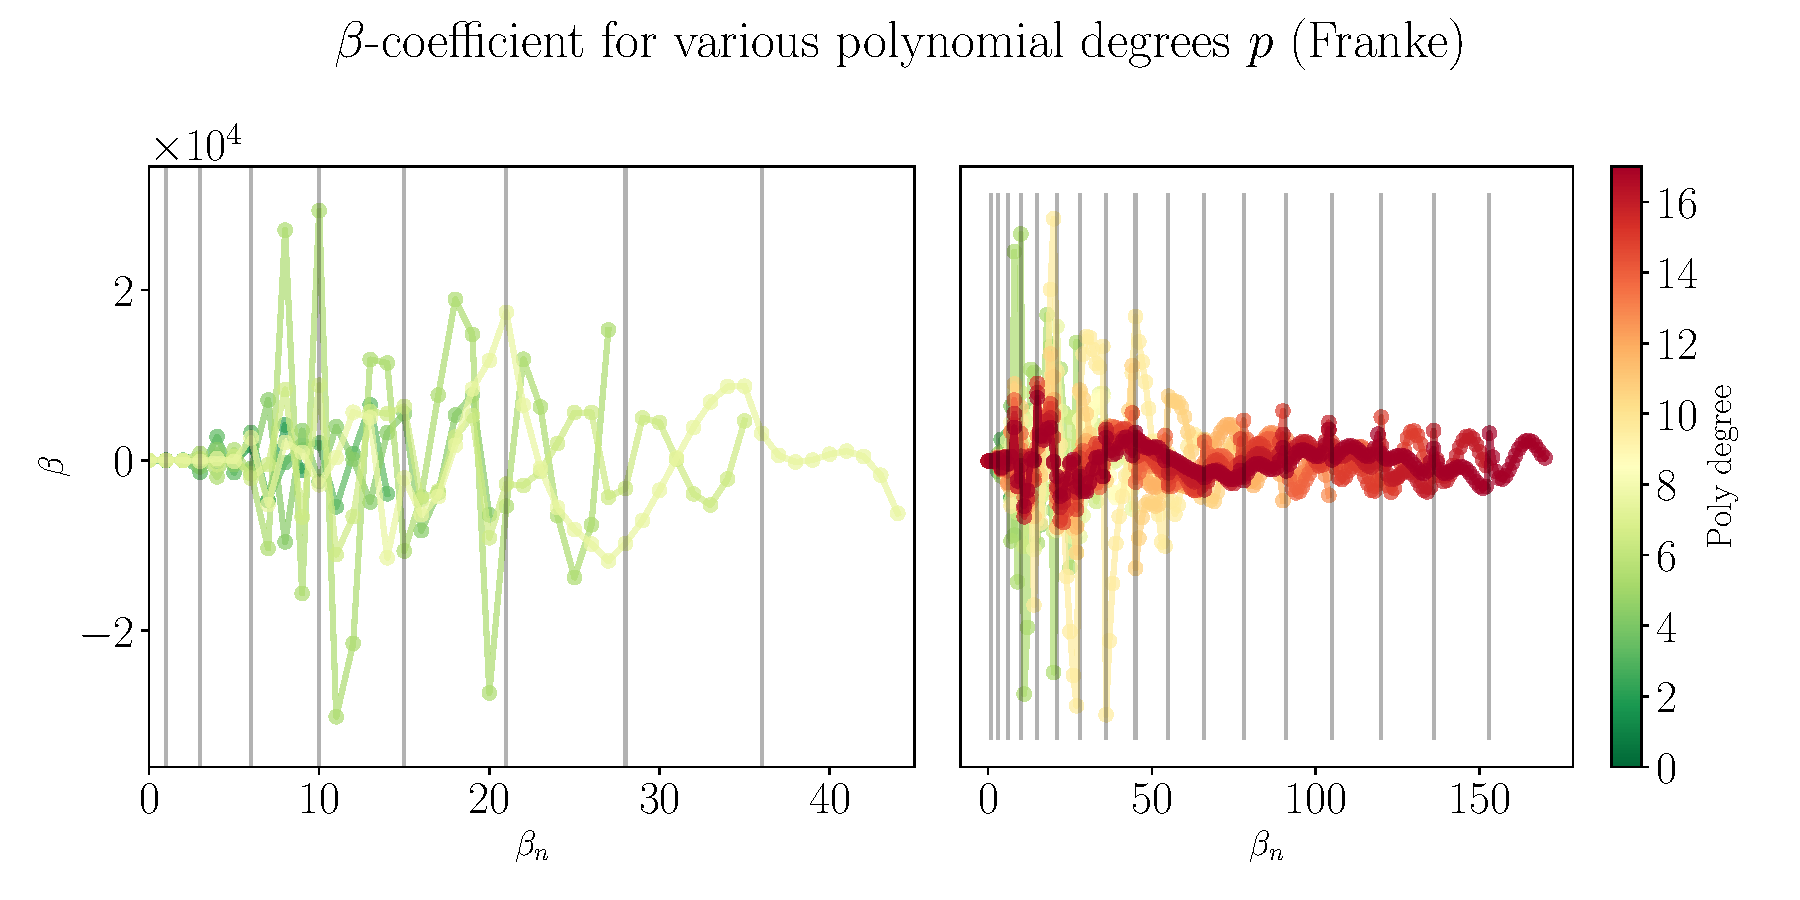
\includegraphics[width=1.15\linewidth]{Python/Figures/OLS/OLS_betano_scaling_1000.pdf}
	\caption{The \(\beta\)-coefficients for the OLS-fit of \(N=1000\) datapoints generated from the Franke function. The plots shows the polynomial degree from 0 (green) to 17 (red). The left hand side is restricted to \(\beta\)-coefficients corresponding to up to \(p=8\). The solid lines in the background indicate where the last coefficient of a given polynomial degree is placed.}
	\label{fig:OLS_beta_degree_1000}
\end{figure}

\subsubsection{Ridge}
This section presents the MSE and \(R^2\)-score for the Ridge regression method using data generated from the Franke function \eqref{eq:franke} given in Fig. \ref{fig:ridge_mse_degree}. These metrics are presented as functions of the polynomial degree \(p\) as before but now with various fixed \(\lambda \)'s. 

Here we can clearly see that there is some discrepancy for different values of $\lambda$. The case where $\lambda=10^{-10}$ can be seen to have its MSE ($R^2$) increase (decrease) quite early on as the polynomial degree increases whilst the cases for larger $\lambda$ remain relatively stable throughout. From the three stable values of $\lambda$ we see that $\lambda=10^{-7}$ and $\lambda=10^{-4}$ perform much better than the others. As such one would expect the optimal $\lambda$ value to lie in between these values. All the MSE and $R^2$ scores can be seen to flatten out as the polynomial degree increases. 
\begin{figure}[ht!]
	\centering
	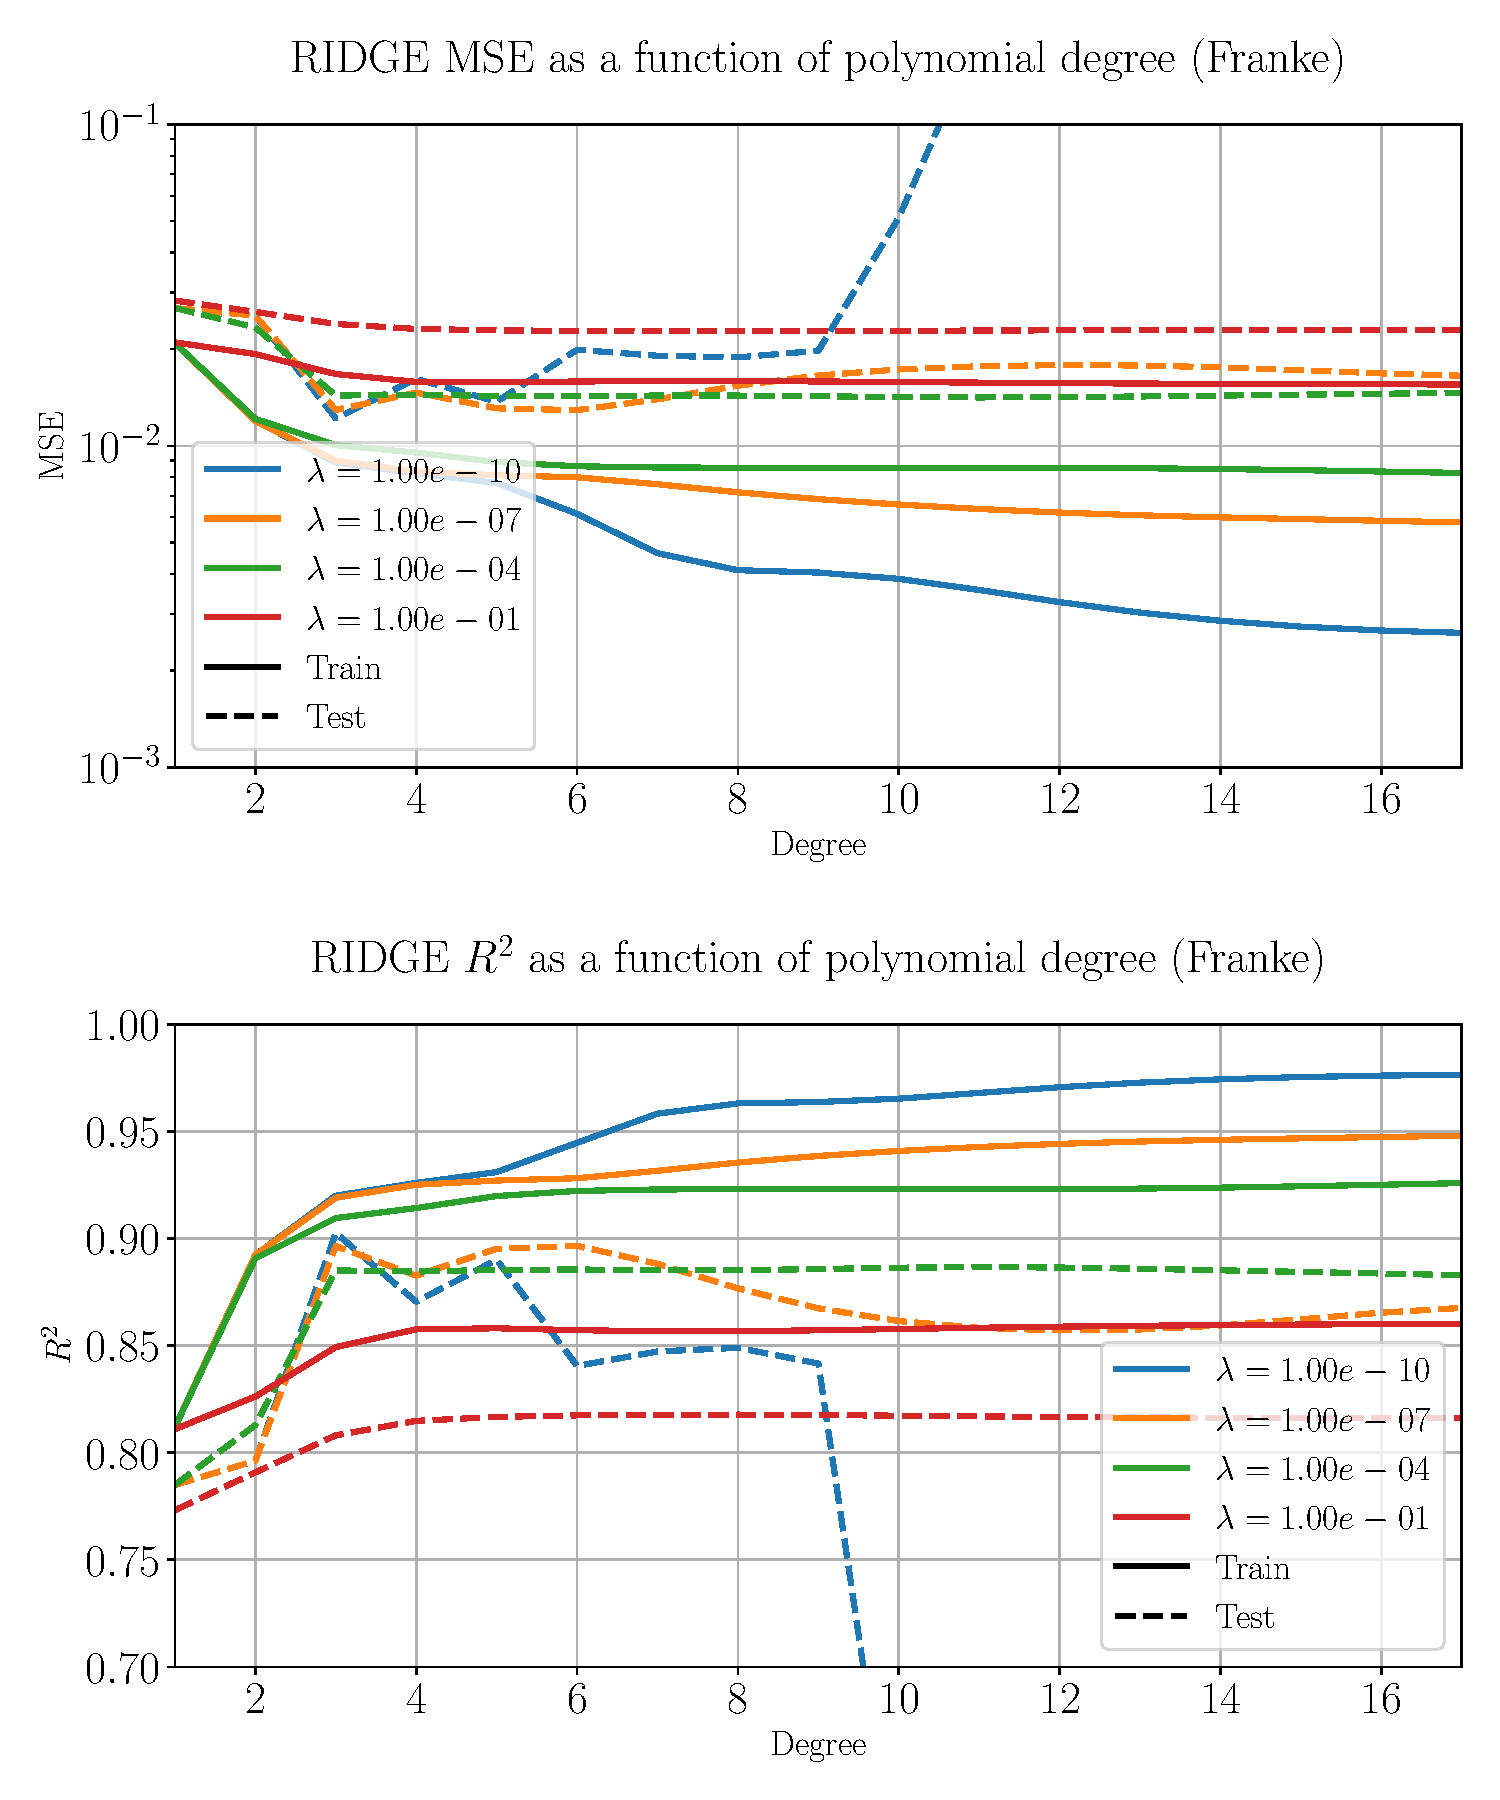
\includegraphics[width=\linewidth]{Python/Figures/Ridge/RIDGE_MSE_R2_Unscaled.pdf}
	\caption{Ridge MSE and $R^2$ as a function of the max polynomial degree with \(p_{\text{max}}=17\). The four chosen values for the hyperparameter $\lambda$ are $10^{-15},10^{-7},10^{-4}$ and $10^{-1}$ which are denoted by the different colors. The solid and dashed lines correspond to the training and test set respectively.}
	\label{fig:ridge_mse_degree}
\end{figure}
This is due to the increased stability Ridge has due to its penalty term. This essentially works to drive down higher order polynomials reducing overfitting. As such Ridge is less sensitive to getting the correct model complexity in place unlike OLS.

To view the dependence on $\lambda$ more explicitly we fixed the degree to \(p=6\) and used 100 logarithmically spaced values of $\lambda$ and plotted the MSE and $R^2$ as a function of $\lambda$ in Fig. \ref{fig:ridge_logMSE_degree}. respectively. The chosen value of $p=6$ was considered due to the diminishing returns from increasing \(p\) past this value, as seen in Fig. \ref{fig:ridge_mse_degree}. These plots suggest an optimal value of $\lambda\sim 10^{-6}$ as this is where the MSE ($R^2$) is the lowest (highest) and is thus the value that was used for further analysis.

\begin{figure}[ht!]
	\centering
	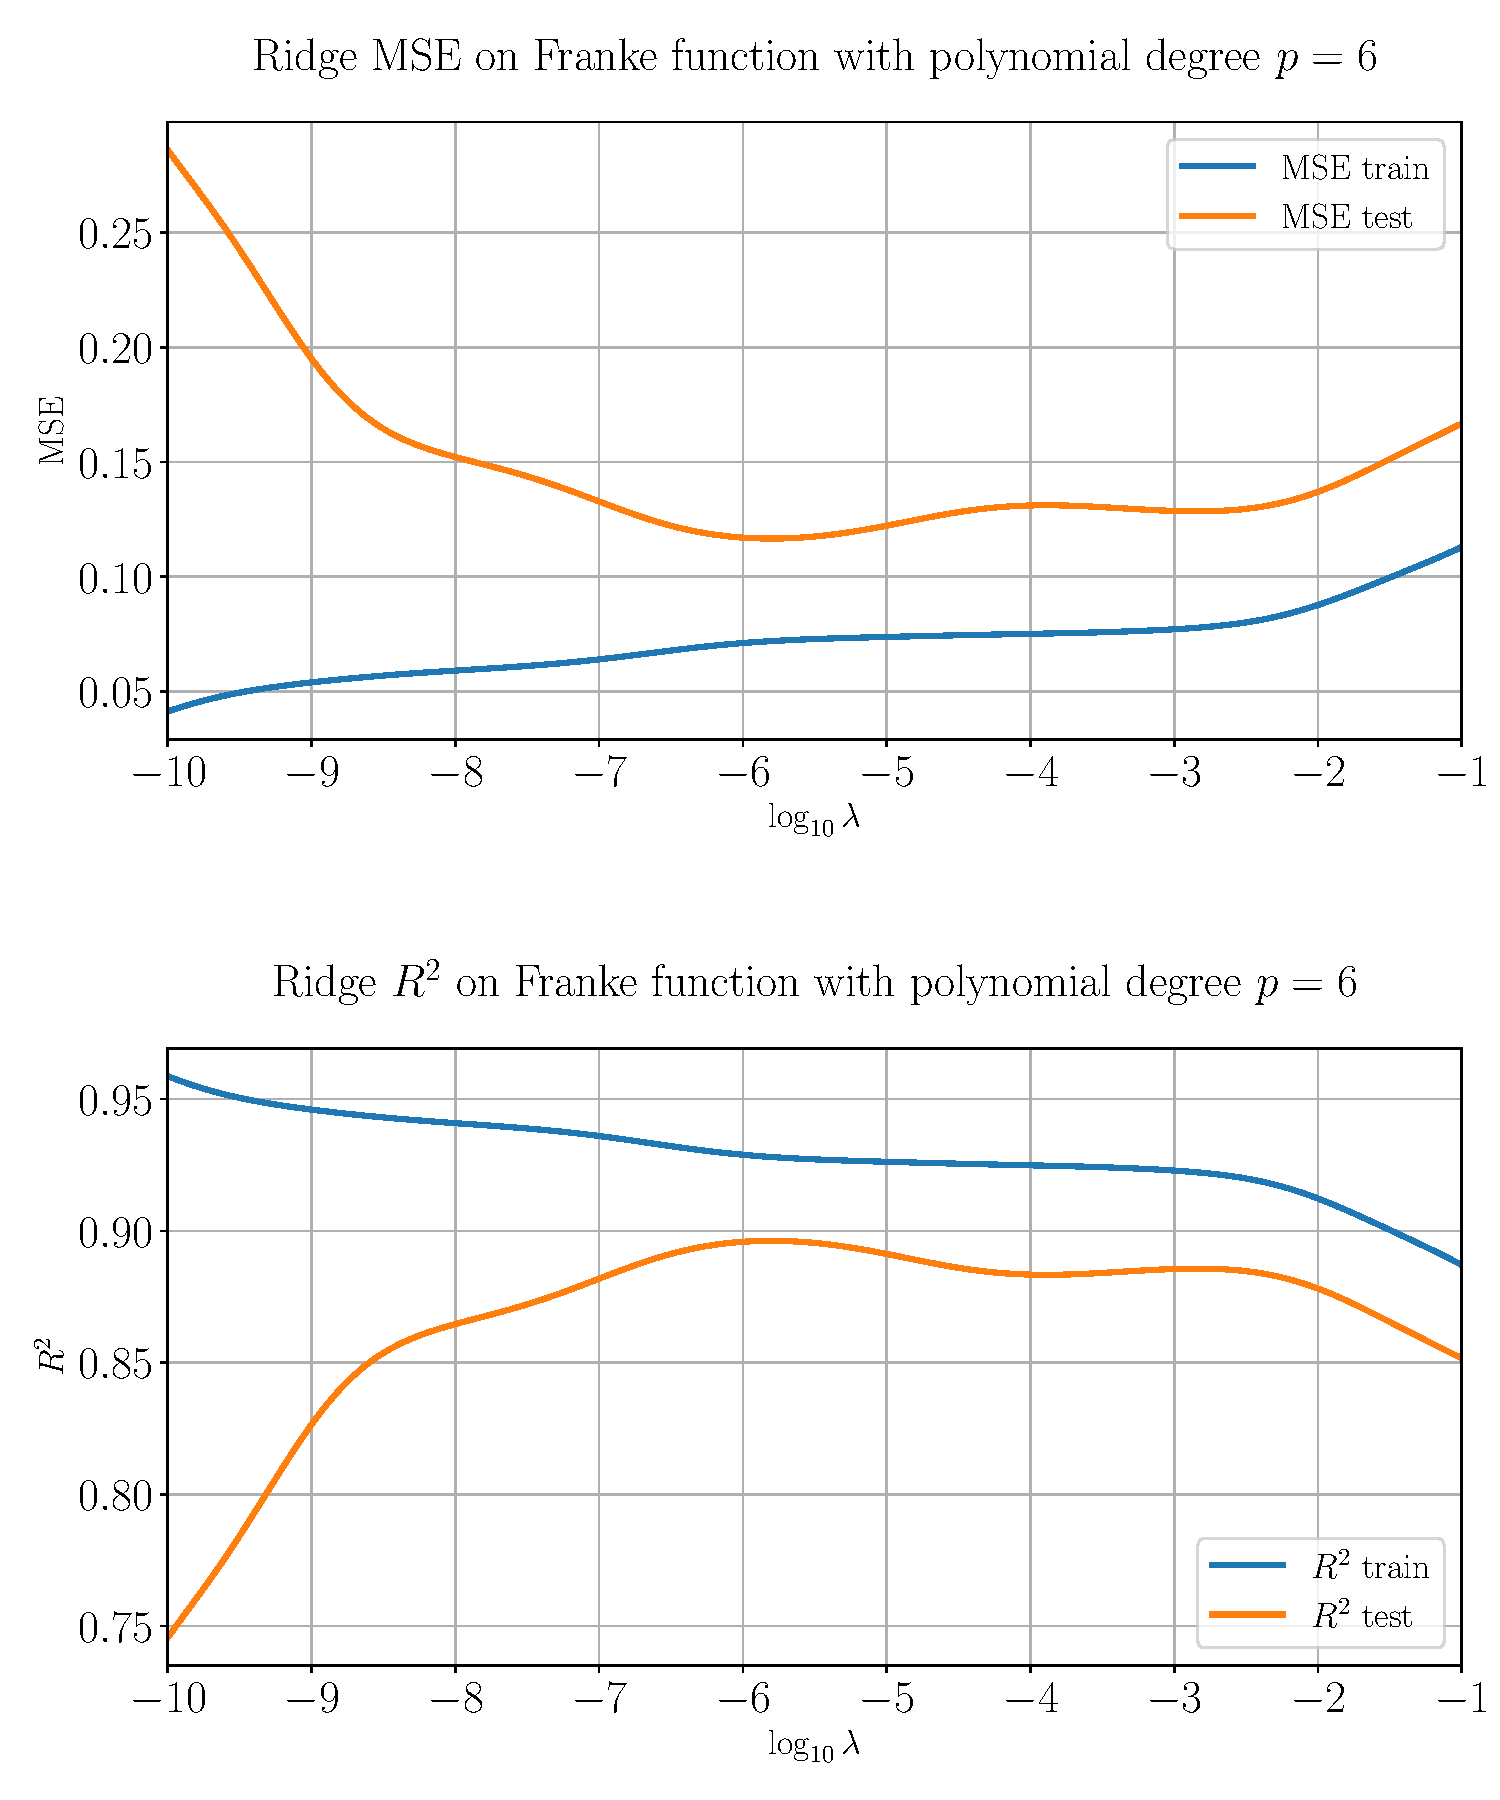
\includegraphics[width=\linewidth]{Python/Figures/Ridge/RIDGE_logMSE_R2_Unscaled.pdf}
	\caption{Ridge MSE and $R^2$ with $p=6$ as a function of the hyperparameter $\lambda$.}
	\label{fig:ridge_logMSE_degree}
\end{figure}

\subsubsection{LASSO}
At last we look at the results for LASSO. Again the MSE and $R^2$-scores as a function of the polynomial degree are given in Fig. \ref{fig:lasso_mse_degree}. Unlike in the cases of OLS and Ridge, these plots are strikingly constant, showing little to no variation. There is a negligible effect on the MSE and \(R^2\)-score from increasing the polynomial degree, and seemingly the only effect of increasing $\lambda$ is to make the MSE ($R^2$) higher (lower). 

\begin{figure}[ht!]
	\centering
	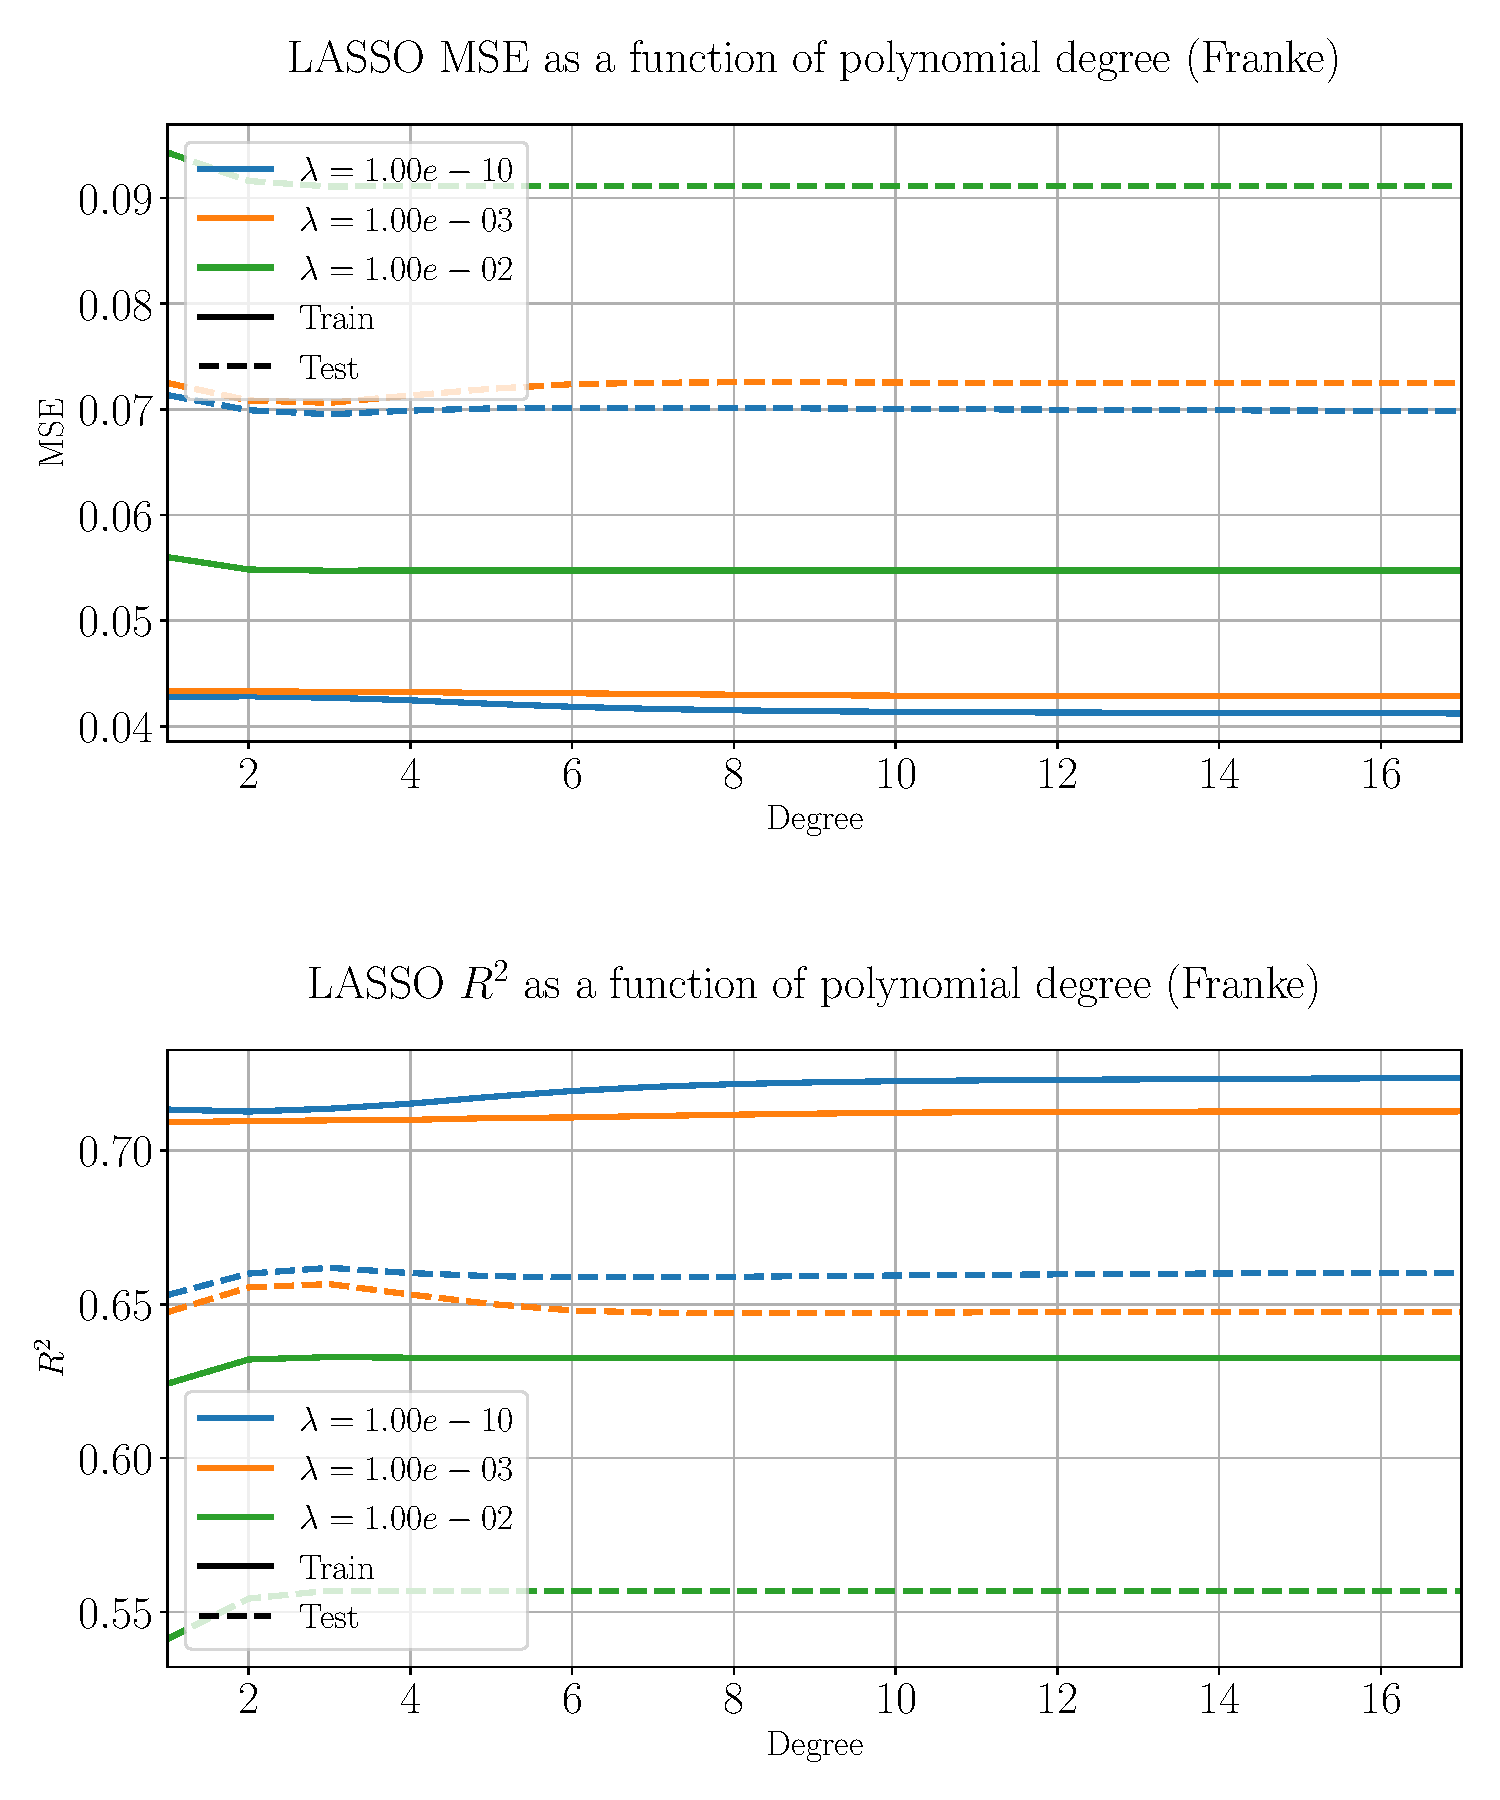
\includegraphics[width=\linewidth]{Python/Figures/LASSO/LASSO_MSE_R2_Unscaled.pdf}
	\caption{LASSO MSE and $R^2$ as a function of the max polynomial degree. The three chosen values for the hyperparameter $\lambda$ are $10^{-10},10^{-3}$ and $10^{-2}$. The remaining description can be found under Fig. \ref{fig:ridge_mse_degree}.}
	\label{fig:lasso_mse_degree}
\end{figure}

This can be seen from Fig. \ref{fig:LASSO_logMSE_degree}. as the two metrics remain close to constant between $\lambda=10^{-10}$ and $\lambda=10^{-3}$. However, for \(\lambda\geq 10^{-3}\), the MSE (\(R^2\)) climbs (falls) almost vertically. The domain \(\lambda\gtrsim 10^{-3}\) is likely when $\lambda$ becomes too large to set crucial $\beta$ coefficients to $0$ and thus causing the method to be underfitting the data.

For the current case the only advantage that LASSO has over OLS is just insensitivity to increase in degree, and thus it is less important to keep the complexity of the model at an optimal level. However Ridge also accomplishes this whilst not massively increasing and decreasing the MSE and $R^2$-score respectively.
\begin{figure}[ht!]
	\centering
	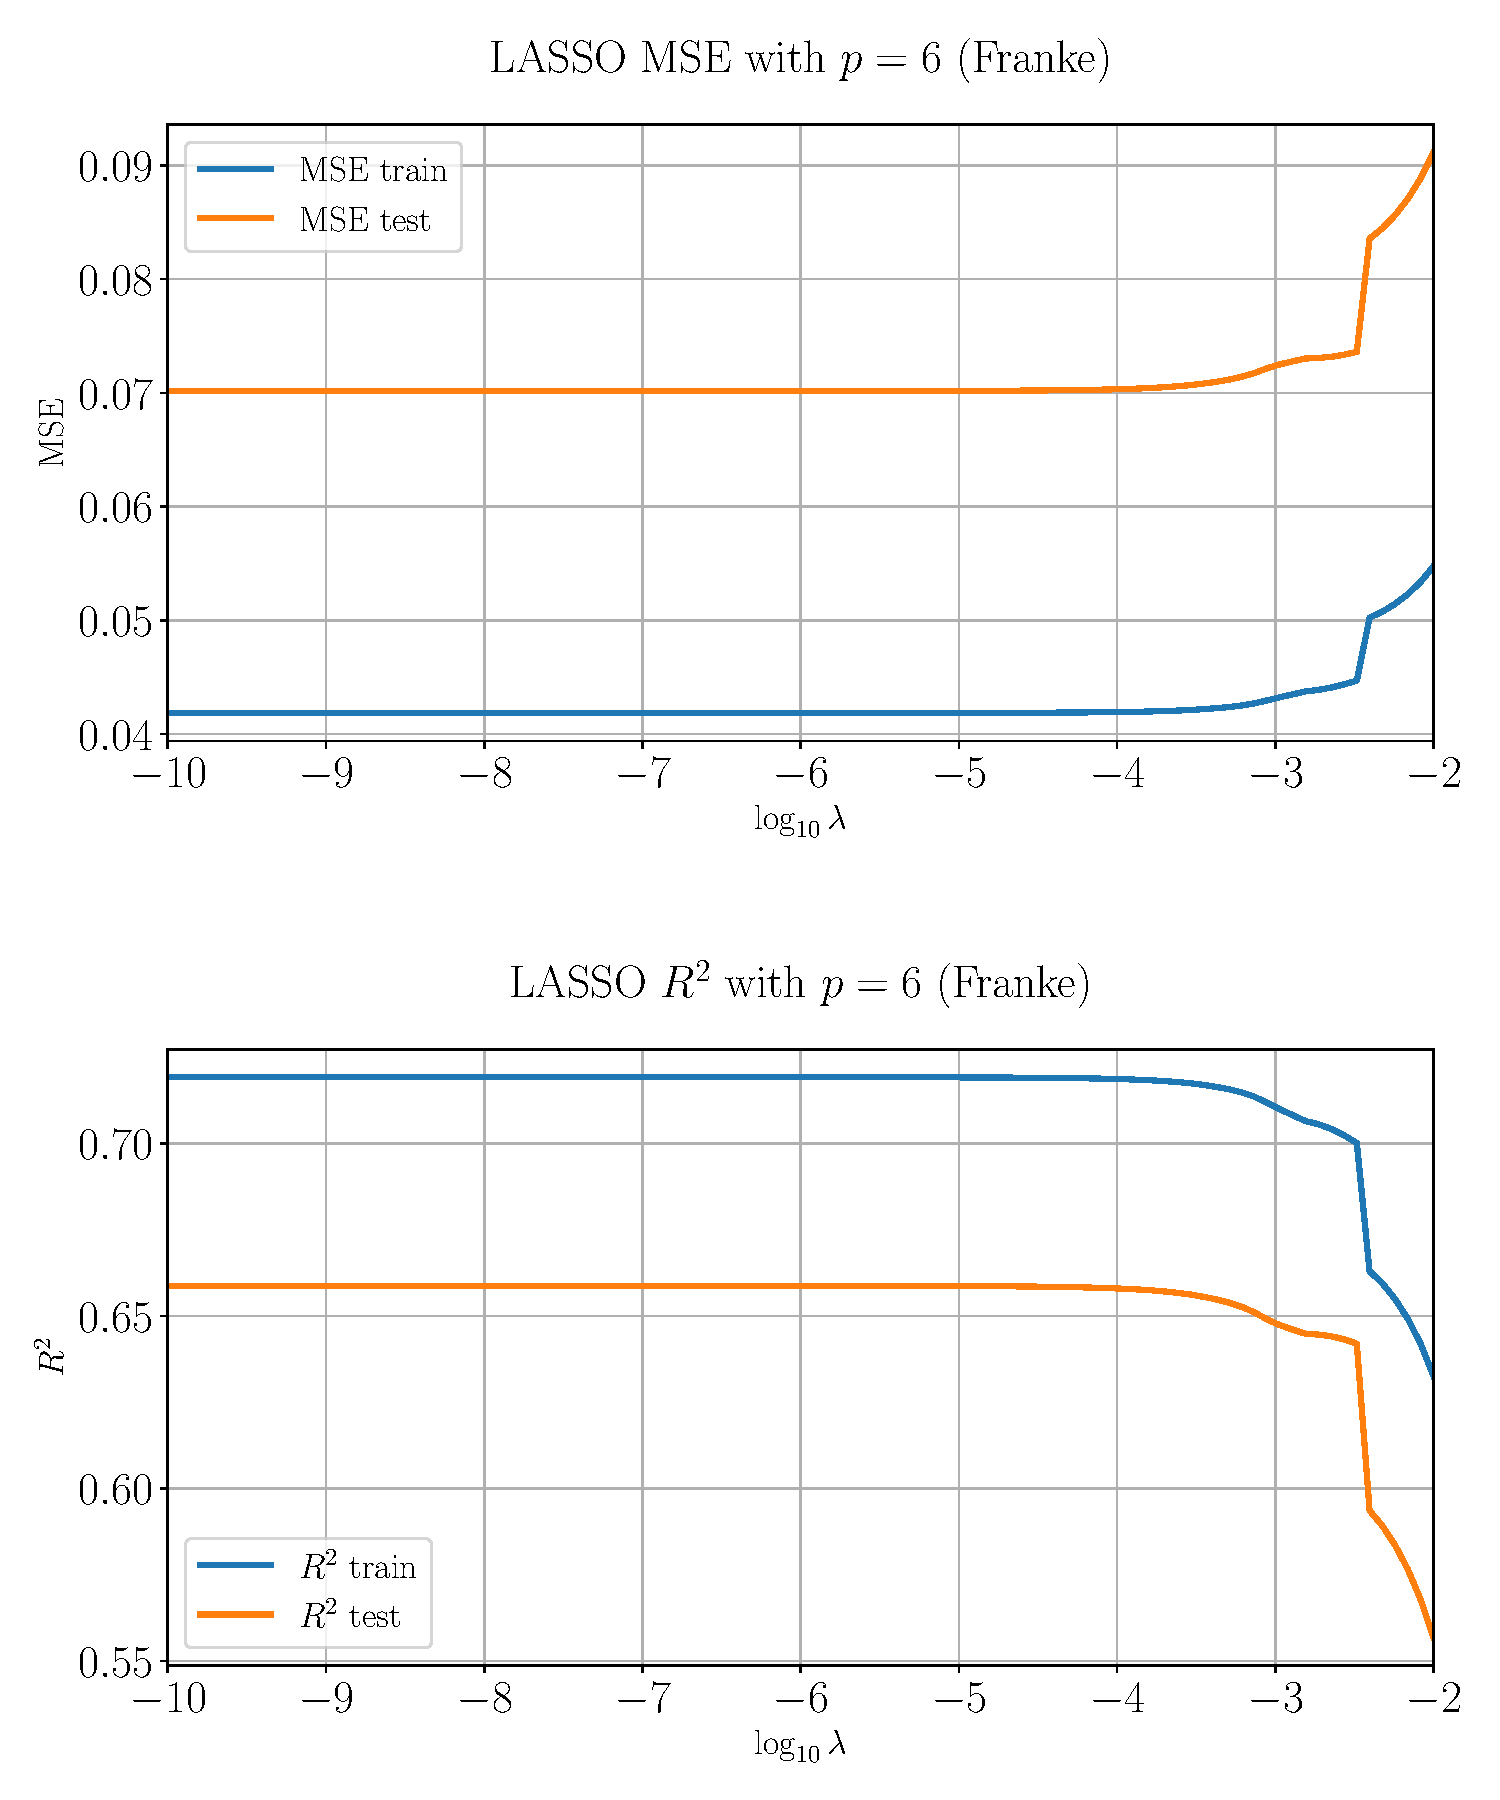
\includegraphics[width=\linewidth]{Python/Figures/LASSO/LASSO_logMSE_logR2_Unscaled.pdf}
	\caption{LASSO MSE and $R^2$ with $p=6$  as a function of the hyperparameter $\lambda$.}
	\label{fig:LASSO_logMSE_degree}
\end{figure}

\subsection{Bootstrap and Cross Validation}
Using the Bootstrap method on the Franke function with OLS regression, $N=25$, $\varepsilon=0.01$ and \(100\) samples, the bias, variance and error is shown in Fig. \ref{fig:bootstrap}. This figure shows a close resemblance to what one would expect from a bias-variance trade-off when compared to e.g. Figure 2.11 in \cite{hastie01statisticallearning}. 

We can see that there is a close-to constant variance for polynomial degrees smaller than \(p\sim7\), whereas for \(p\gtrsim 7\) the variance increases steadily. On the other hand, the bias starts out above \(\sim0.1\), gradually decreasing, reaching a minimum for \(p\) in the range \(4-9\), before rising again for \(p\gtrsim 9\). These specific values of \(p\) is dependent on the sample size \(N=25\) and the amount of samples taken by the Bootstrap method. However, the general shape of the error curve in Fig. \ref{fig:bootstrap} is expected to be independent of these settings. Due to the choice of $\sigma^2=0.01$ the error is supposed roughly equal to the sum of the variance and the bias, as seen in \eqref{eq:MSE-bias-var}. Visually, Fig. \ref{fig:bootstrap}. confirms this, although the sum is not explicitly given. This figure shows explicitly how underfitting the data gives a large bias and overfitting it introduces a large variance as was eluded to in the theory section.

\begin{figure}[ht!]
	\centering
	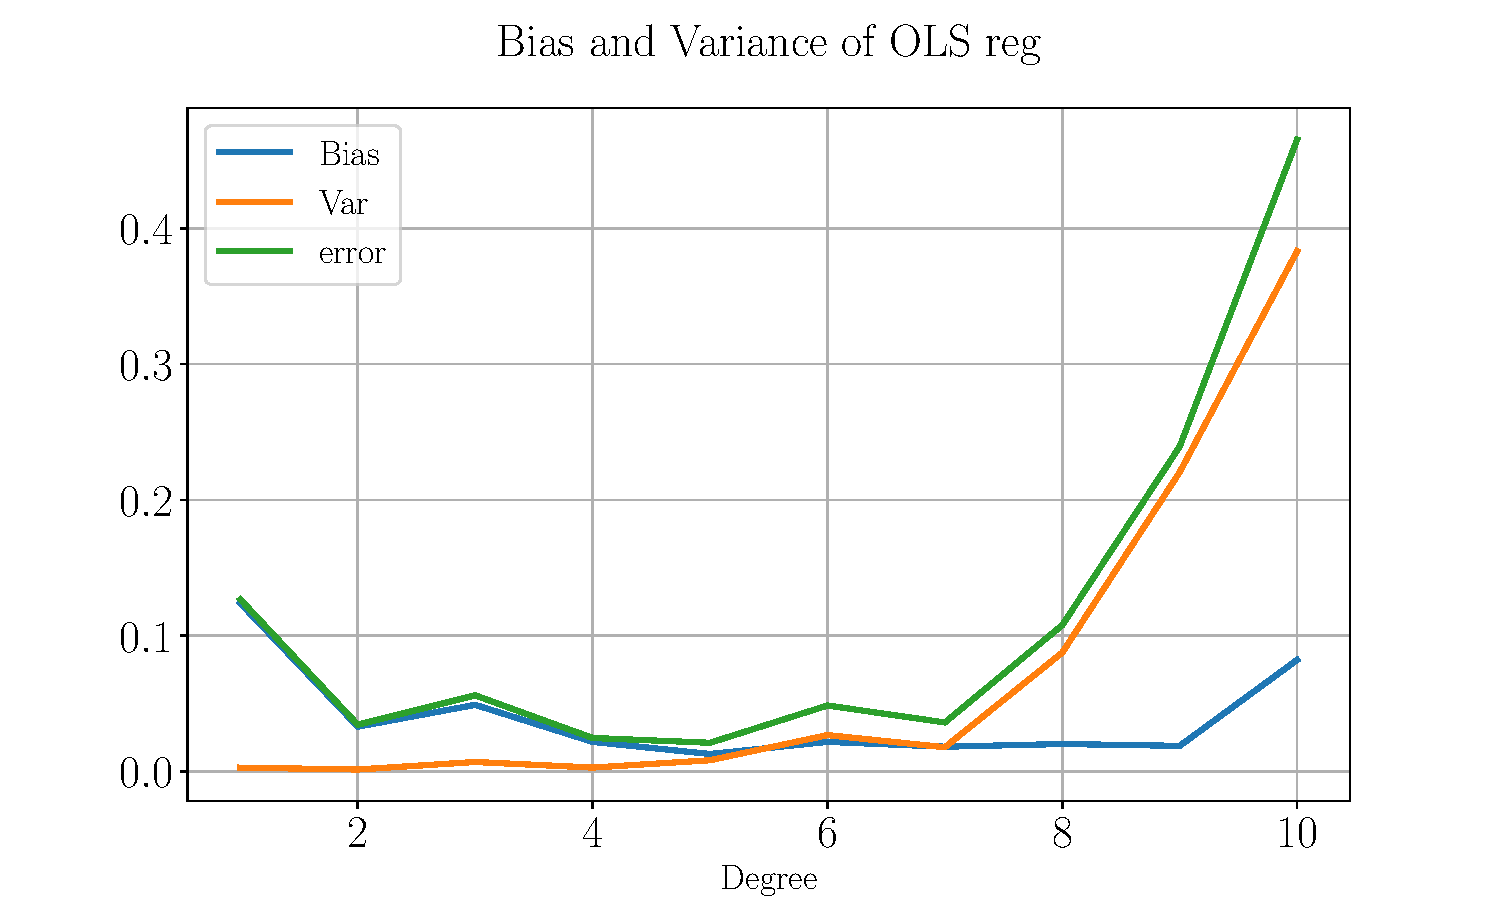
\includegraphics[width=\linewidth]{Python/Figures/OLS/OLS_Bootstrap_BiasVar_no_scaling_GOOD.pdf}
	\caption{The bias, variance and error of a OLS regression on data generated from \(N=25\) samples of the Franke function with noise proportional to \(\varepsilon=0.01\). The metrics are generated using the bootstrap method.}
	\label{fig:bootstrap}
\end{figure}
The MSE and $R^2$ for the three regression methods using $k$-fold Cross validation with \(\lambda=10^{-6}\) and $k=10$ on data generated from the Franke function are given in Fig. \ref{fig:Franke_MSE_CV}. The error bars here show the standard deviation calculated from the $10$-folds used. Here we see that for this remains much more stable across higher polynomial degrees where both OLS and Ridge are mostly flat throughout unlike in the previous cases. We see that in the $R^2$ figure that there is a downwards spike for LASSO at $p=6$. It is not immediately clear what is causing this as from the MSE there is nothing suggesting that this particular polynomial degree gives a much worse fit and is seemingly only an effect on this particular seed. Ignoring this artifact it is still rather clear that LASSO performs overall worse than both OLS and Ridge. Overall it seems that $p=4$ gives the best fit for OLS whilst Ridge performs equivalently well for many of the different polynomials. For simplicity one would then simply pick the lowest order polynomial degree which gives the best result.
\begin{figure}[ht!]
	\centering
	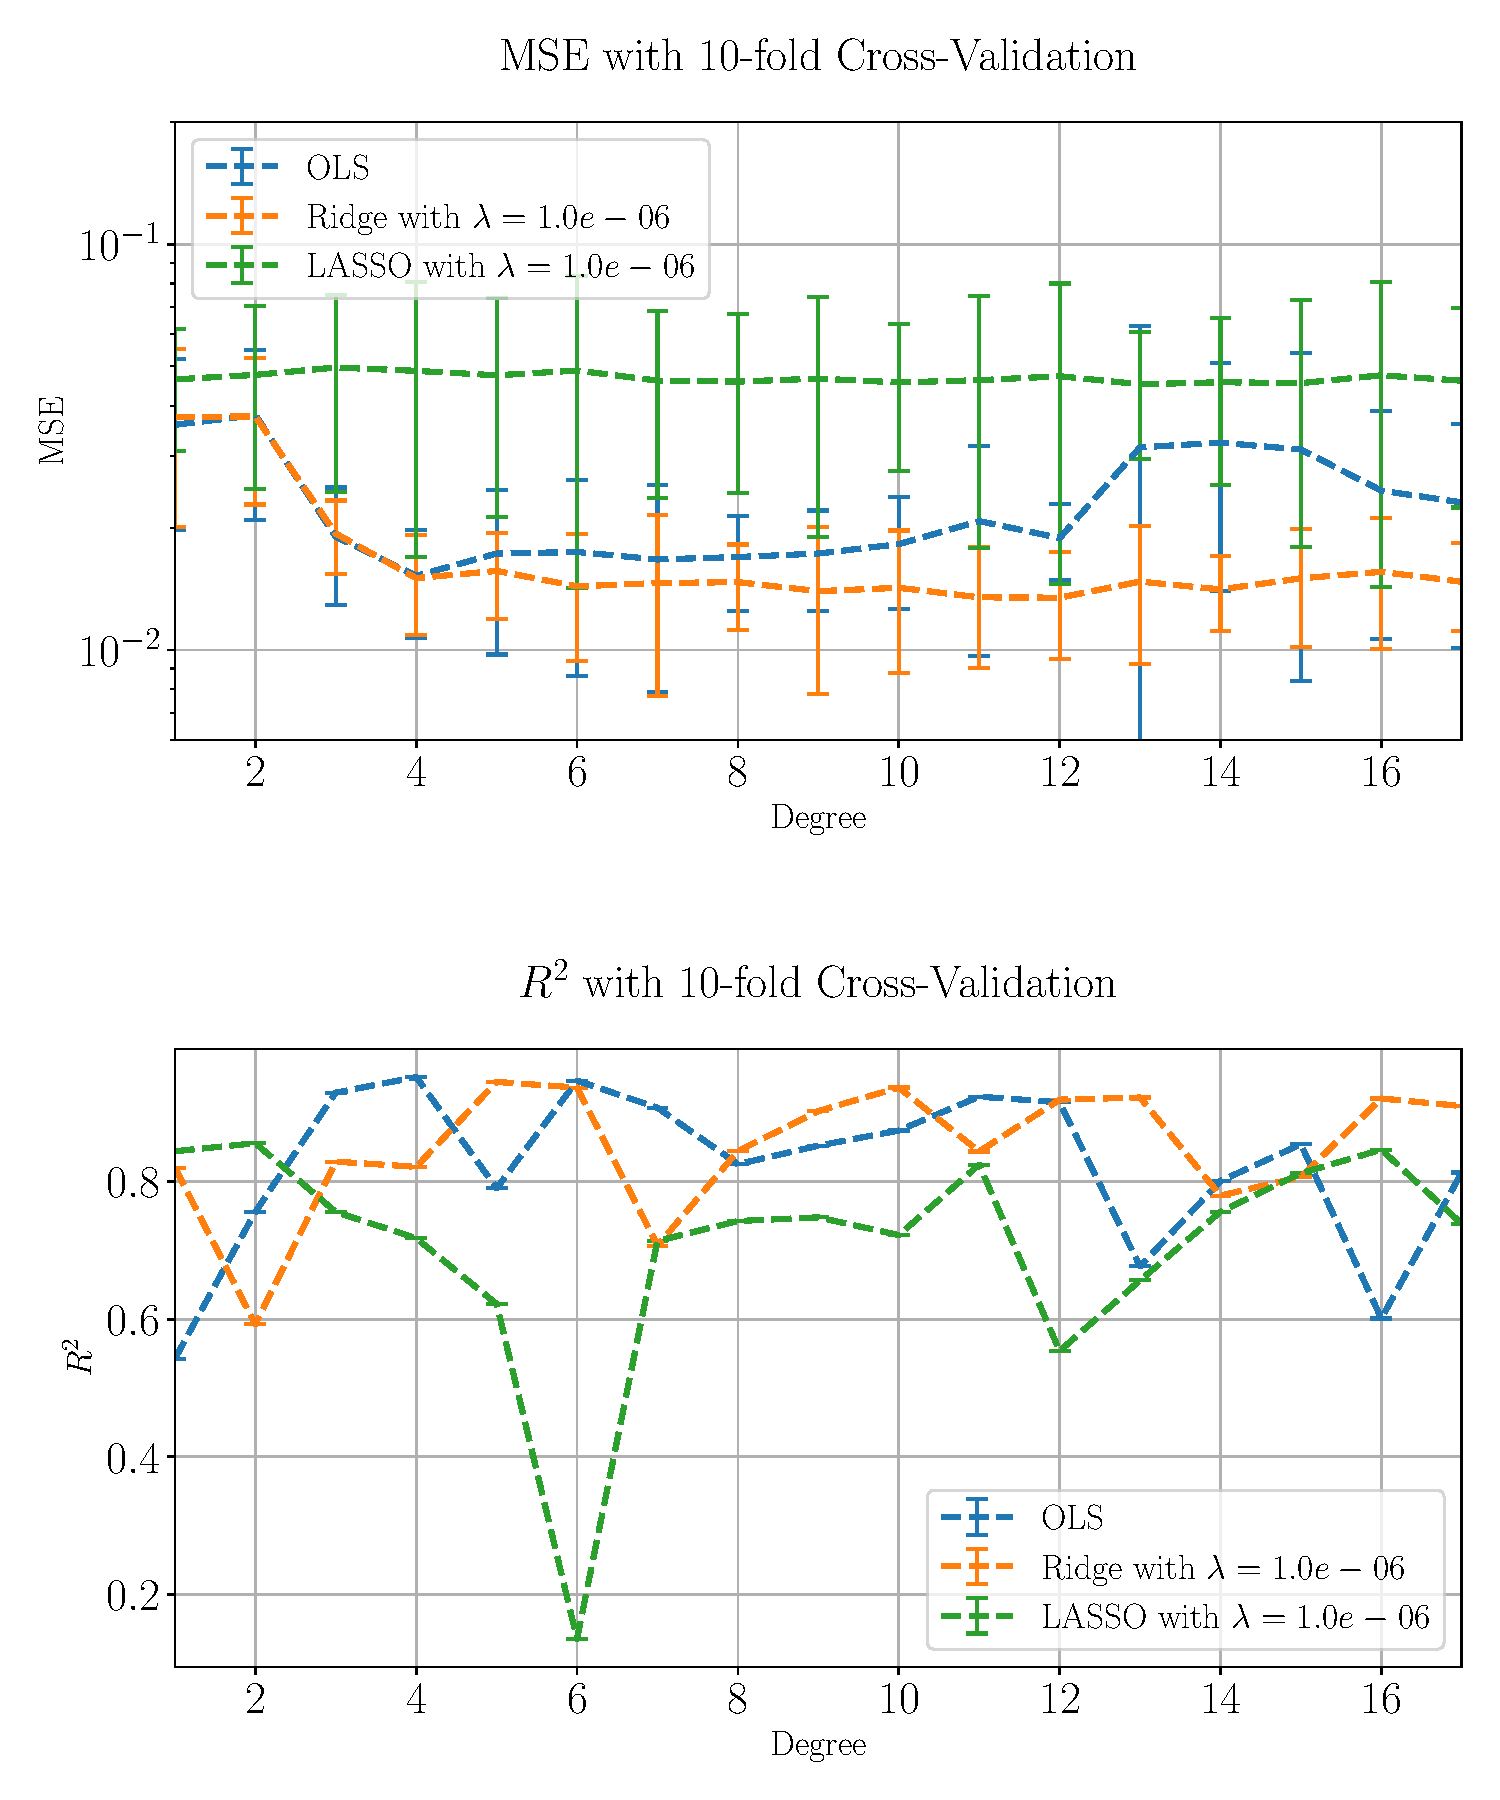
\includegraphics[width=\linewidth]{Python/Figures/CV/CV_MSE_R2_Unscaled_0.pdf}
	\caption{MSE and $R^2$ with 10-fold Cross validation for the three methods as a function of the polynomial degree on data generated from the Franke function. The $y$-axis shows the MSE with error-bars for the three methods, with \(\lambda=10^{-6}\). }
	\label{fig:Franke_MSE_CV}
\end{figure}

\subsection{Terrain Data}
% Contourplots of Grand Canyon and Mount Everest are shown in fig. \ref{fig:GC_ME_Image_Contour}. As can be seen 
The MSE of all the three regression methods OLS, Ridge and LASSO with \(\lambda=10^{-2}\) and standard scaling is shown in \ref{fig:MSE_GrandCan_StandardScaling_17} and \ref{fig:MSE_MountEve_StandardScaling_17} using cross validation, for Grand Canyon and Mount Everest, respectively. As mentioned prior, due to computational purposes we have chosen to work with only a small subsection of the full data. In particular we only work with $N=11$ points as the program already begins to slow down heavily due to the high polynomial degree required. 
% Countourplots of Grand Canyon and Mount Everest can be seen in \ref{fig:GC_ME_Image_Contour}, which suggest a greater complexity than that of the Franke function, comparing to \ref{fig:frankefunction}. 
Both figures show the cross validated Ridge and OLS following each other until OLS increases, jaggedly and with greater error bars, away from Ridge. LASSO on the other hand, slowly decreases, seemingly reaching a constant value as \(p\) increases, above Ridge. The MSE of Mount Everest is greater for low order polynomials, while Grand Canyon seem to favor higher order polynomials. Visually, the lowest MSE is found with Ridge and a polynomial degree in the approximate range \(p\in[11, 15]\), \(p\in[4,6]\) for Grand Canyon and Mount Everest, respectively. 
% In Grand Canyon we do not map the parts with large cliffs but instead mostly flatland. Thus one may expect a lower order polynomial regression performs relatively good here.
\begin{figure}[H]
	\centering
	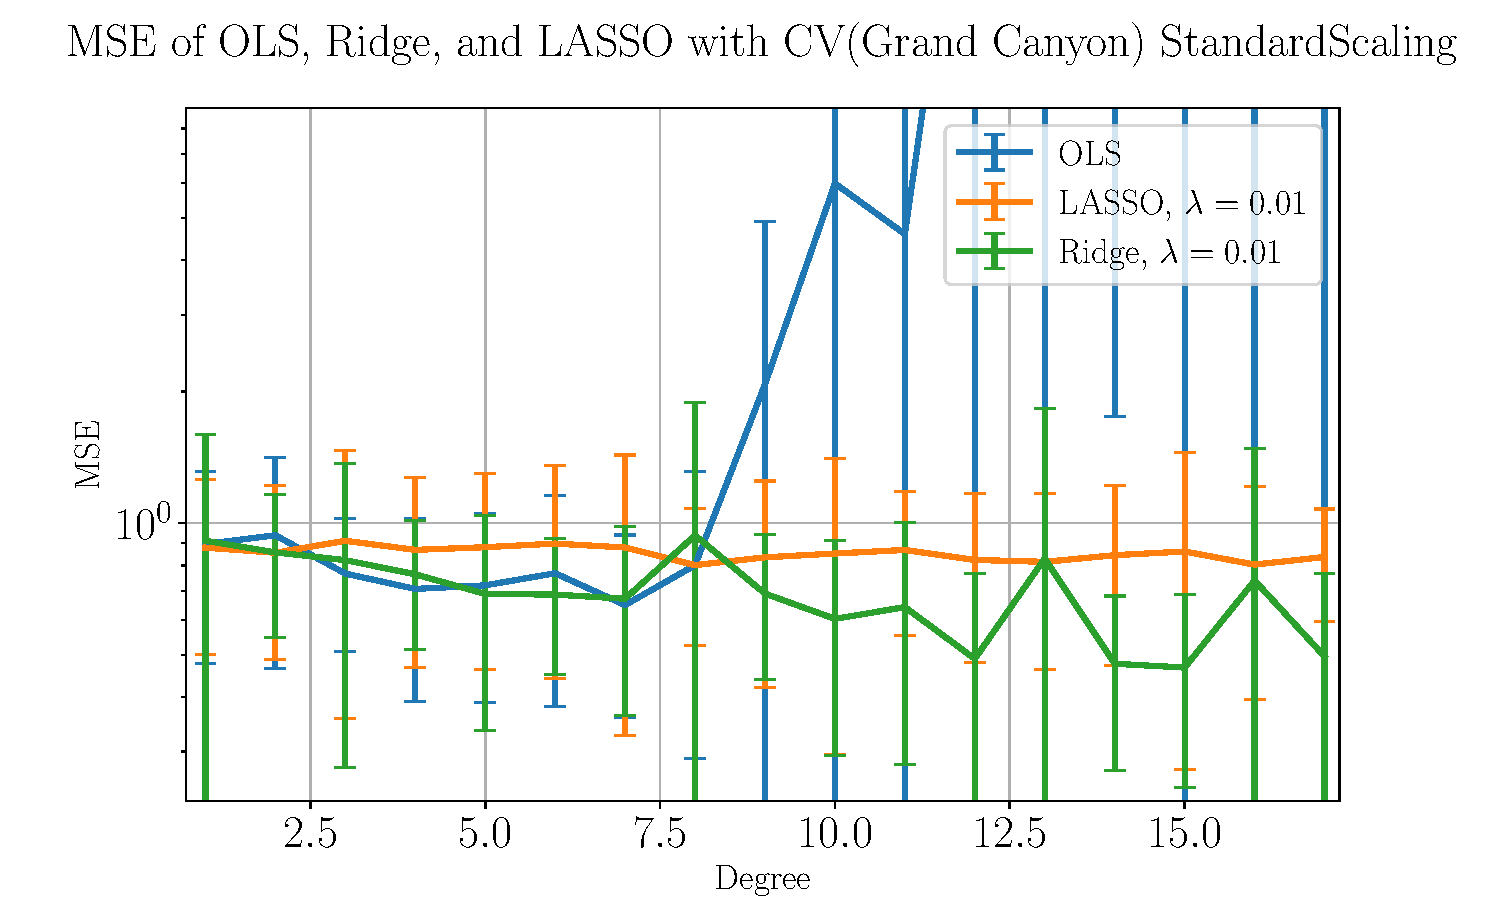
\includegraphics[width=\linewidth]{Python/Figures/Terrain/MSE_GrandCanyon_StandardScaling_17.pdf}
	\caption{MSE of Grand Canyon terrain data from \cite{USGS_EarthExplorer} with 10-fold cross-validation as a function of polynomial degree $p$ for all three regression methods. The error-bars show the standard deviation resulting from the 10 folds.}
	\label{fig:MSE_GrandCan_StandardScaling_17}
\end{figure}

\begin{figure}[H]
	\centering
	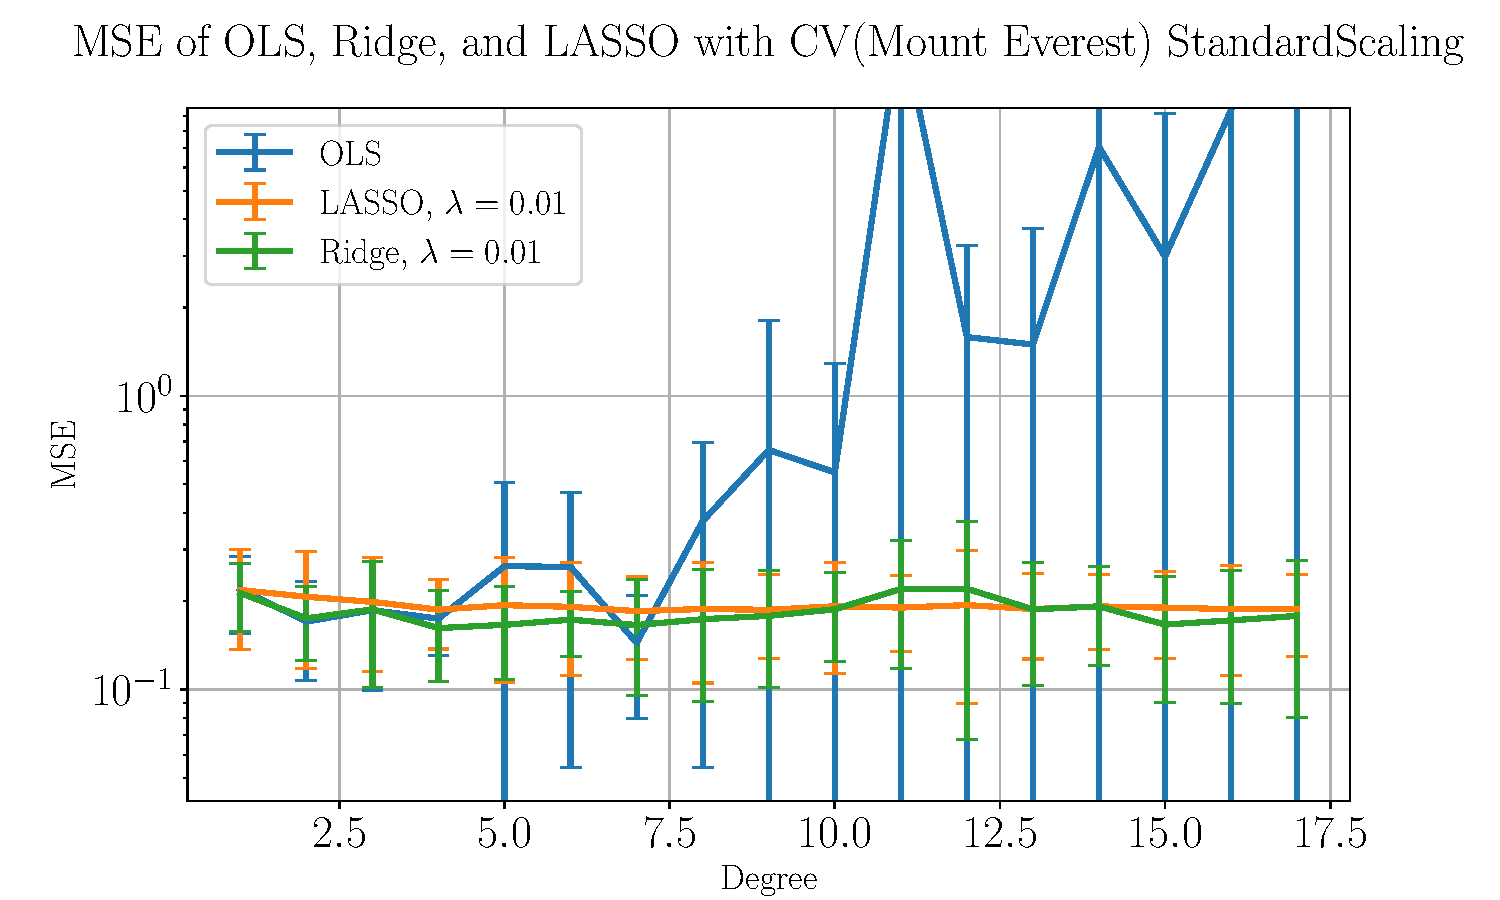
\includegraphics[width=\linewidth]{Python/Figures/Terrain/MSE_MountEverest_StandardScaling_17.pdf}
	\caption{MSE of Mount Everest terrain data from \cite{USGS_EarthExplorer} with 10-fold cross-validation as a function of polynomial degree $p$ for all three regression methods. The error-bars show the standard deviation resulting from the 10 folds.}
	\label{fig:MSE_MountEve_StandardScaling_17}
\end{figure}

Figs. \ref{fig:log_GrandCan_StandardScaling_10} and \ref{fig:log_MountEve_StandardScaling_10} show the MSE and $R^2$ of Ridge and LASSO as a function of \(\lambda\) with \(p=10\), \(p=4\) for the Grand Canyon and Mount Everest respectively. In the case of Grand Canyon, Fig. \ref{fig:log_GrandCan_StandardScaling_10} suggests that Ridge, with an \(\lambda\)-value of \(\sim 1e-7\), gives the best MSE. For Mount Everest, it seems both Ridge and LASSO are constant for \(\lambda\in[10^{-10}, 10^{-3}]\), with Ridge outperforming LASSO.

\begin{figure}[H]
	\centering
	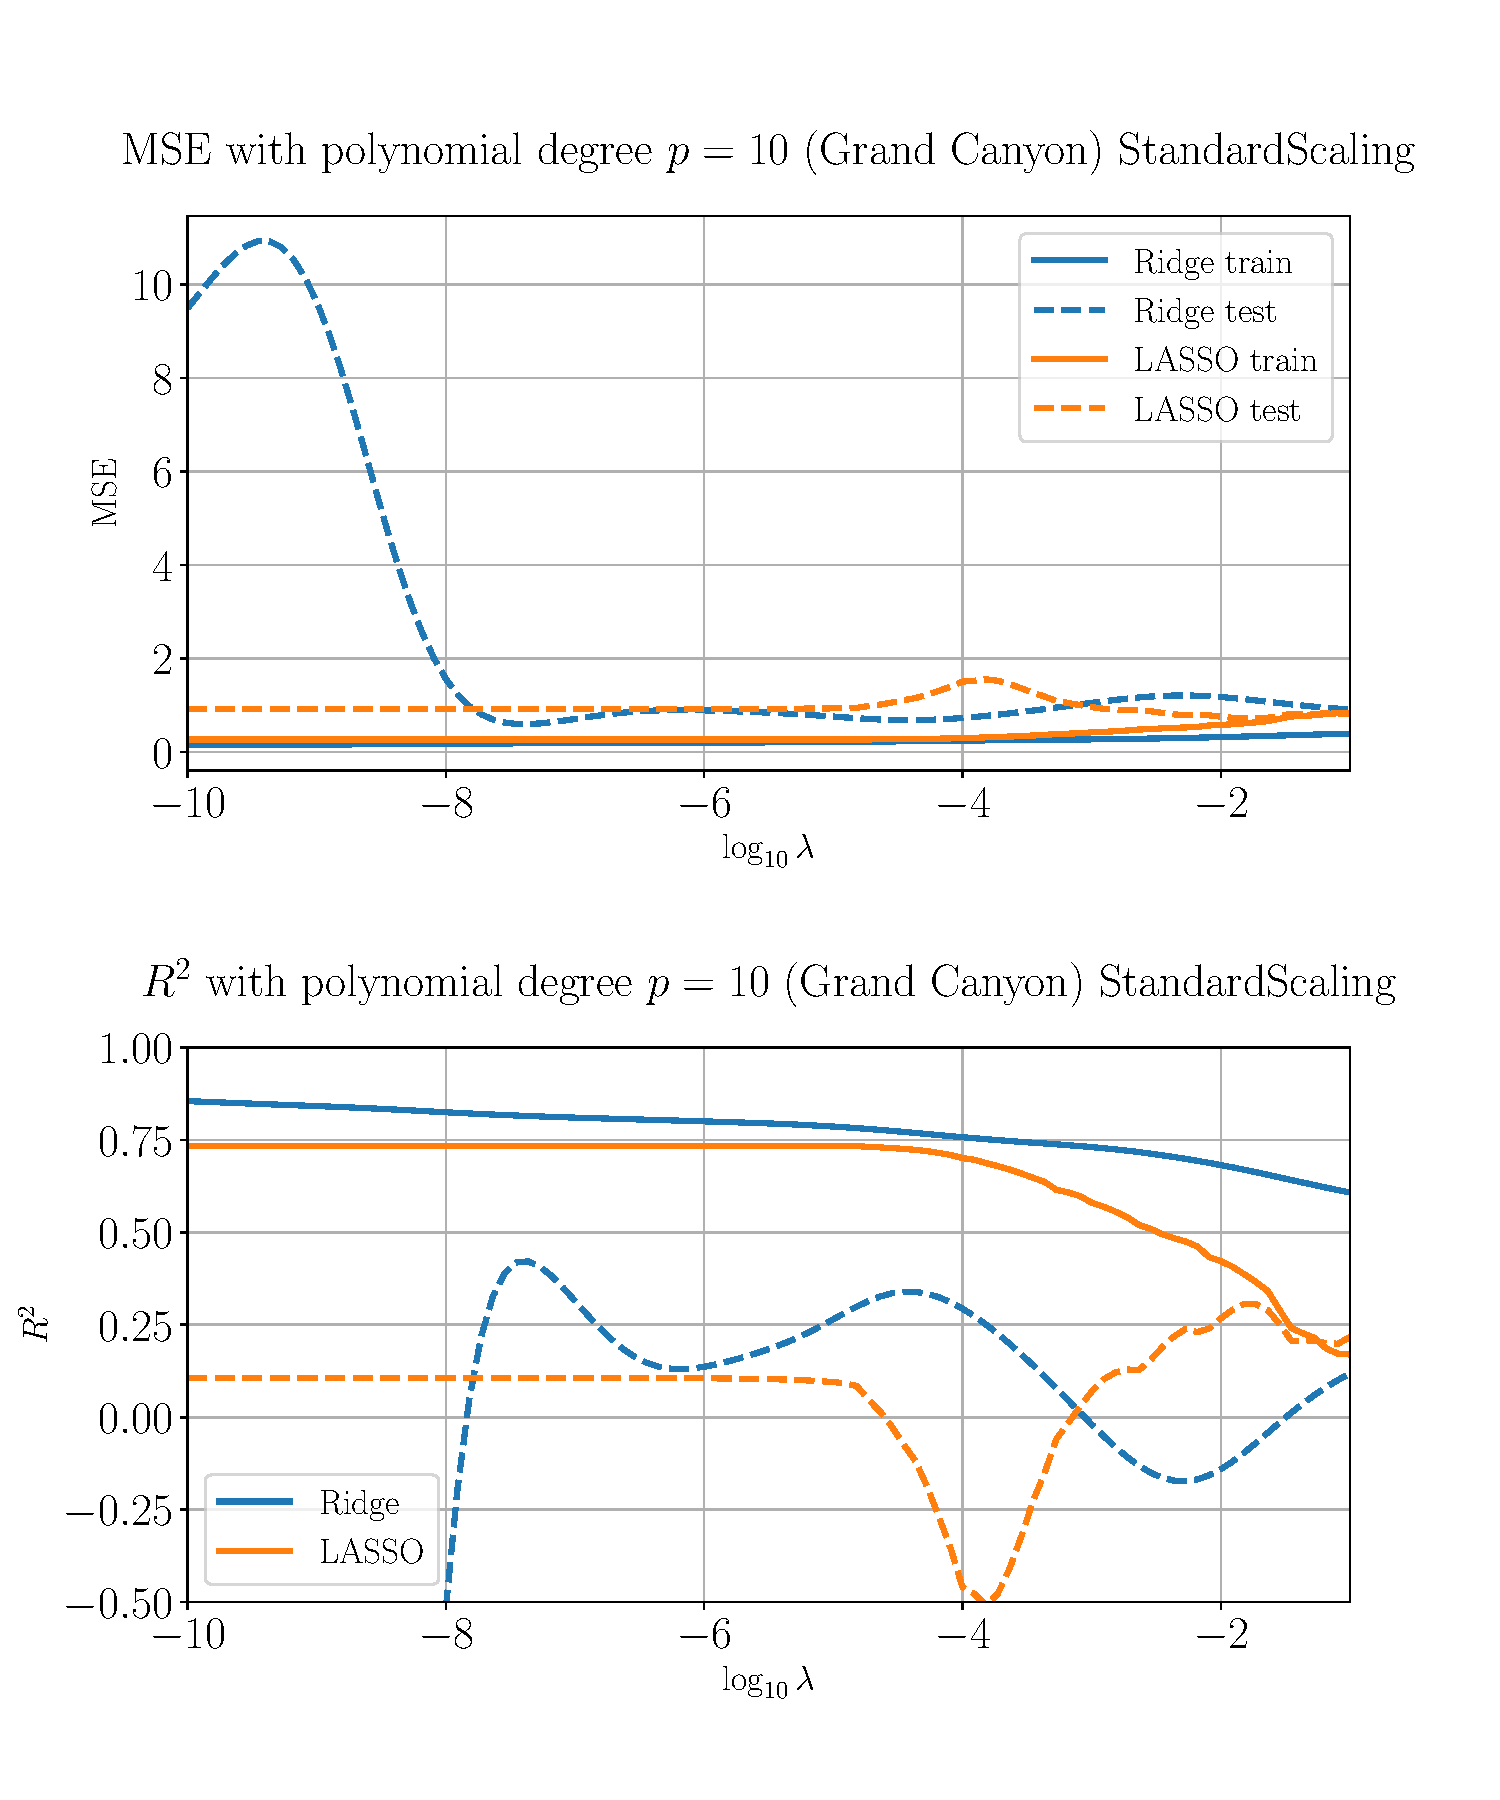
\includegraphics[width=0.95\linewidth]{Python/Figures/Terrain/log_MSE_R2_GrandCanyon_StandardScaling_10.pdf}
	\caption{MSE and $R^2$ of Grand Canyon terrain data with $p=10$ for Ridge and LASSO as a function of the hyperparameter $\lambda$.}
	\label{fig:log_GrandCan_StandardScaling_10}
\end{figure}

\begin{figure}[H]
	\centering
	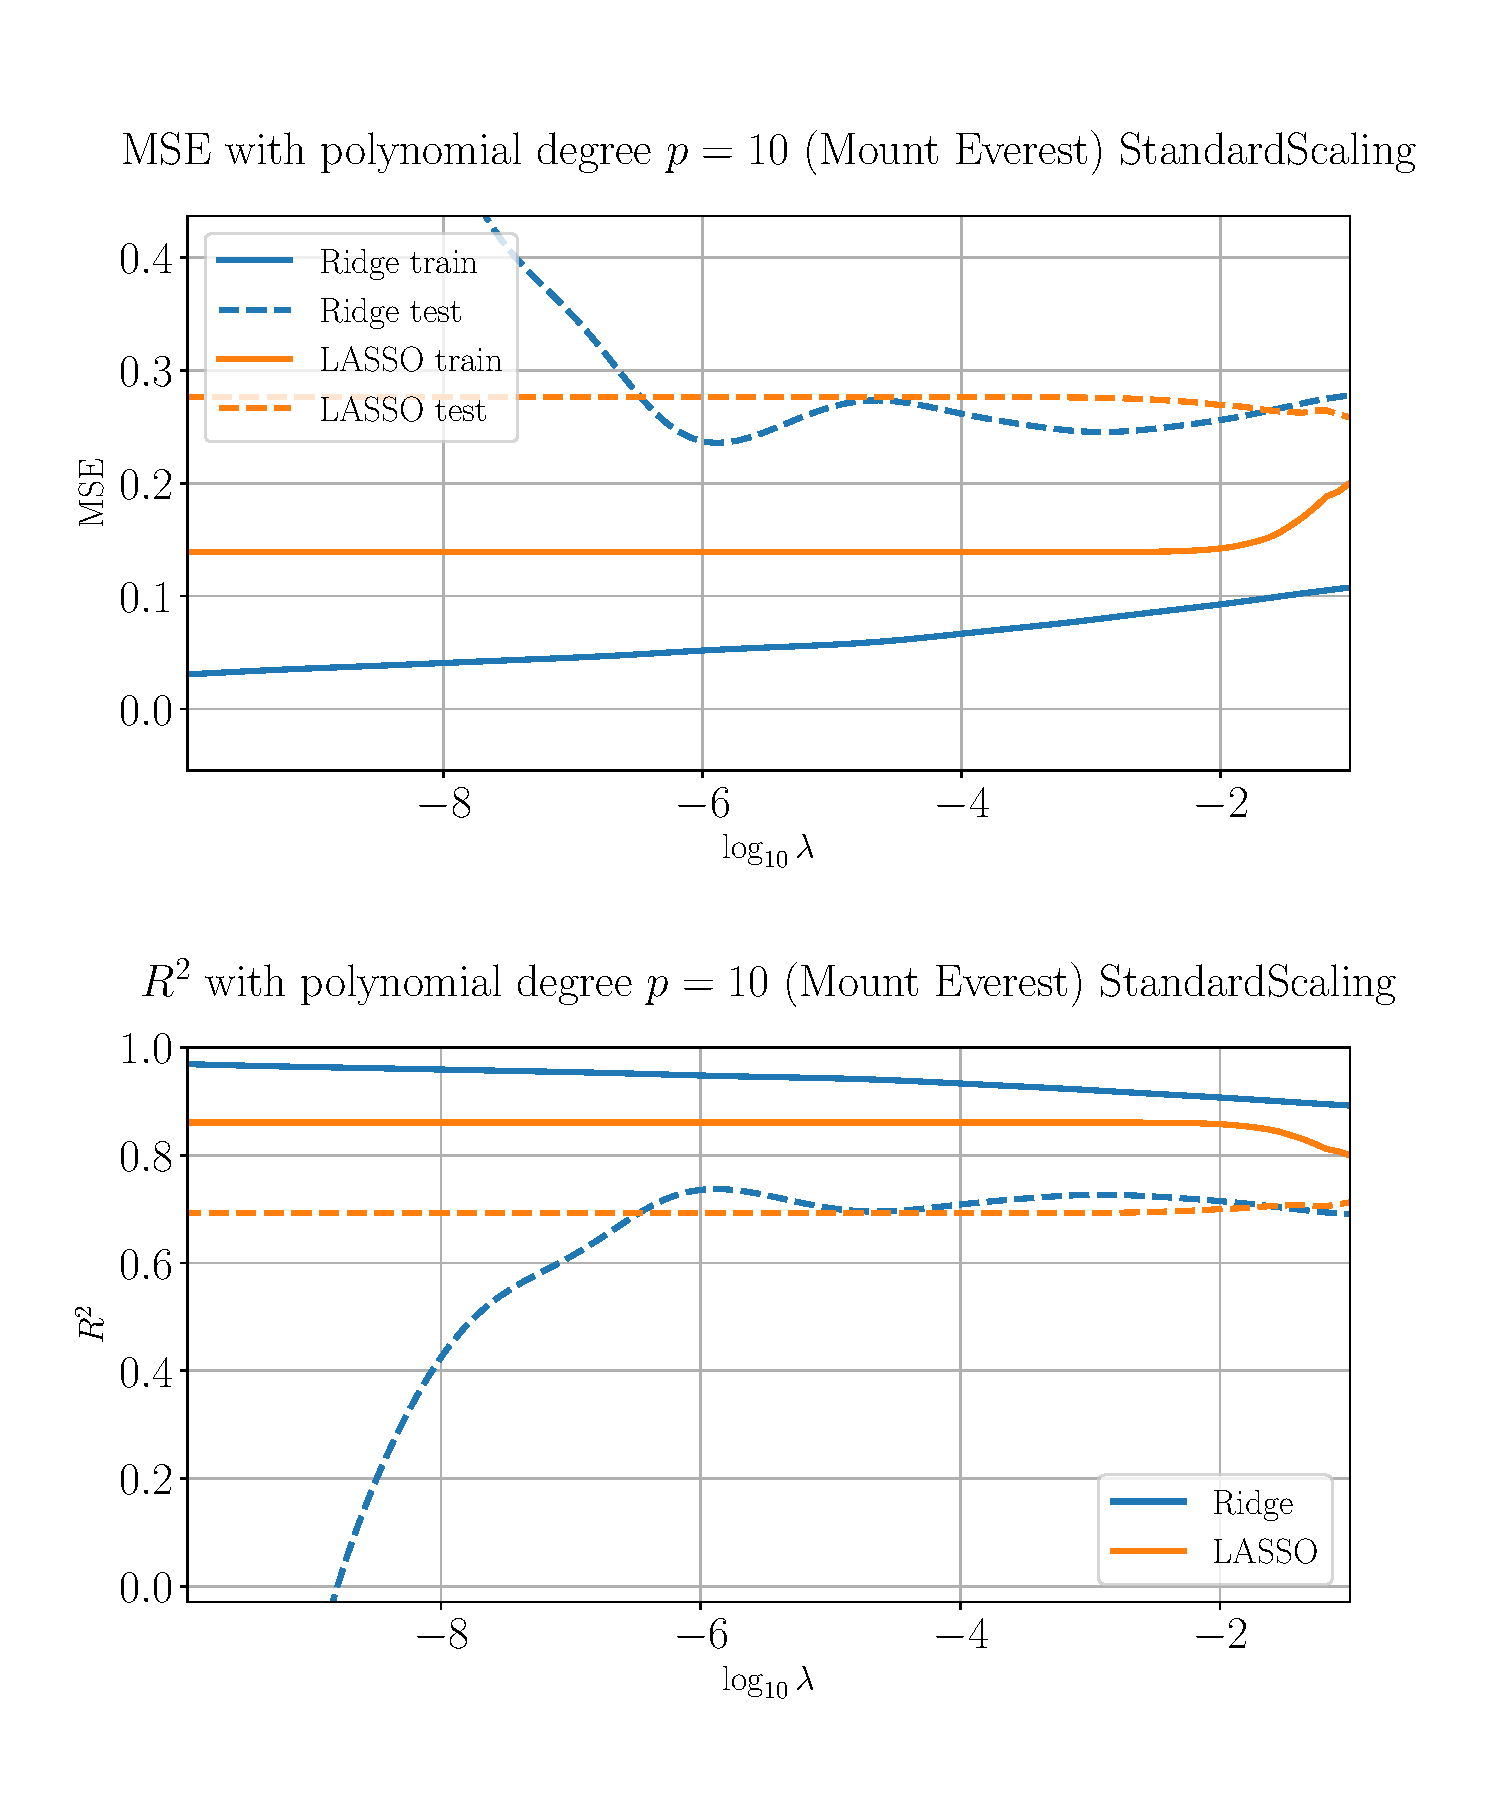
\includegraphics[width=0.95\linewidth]{Python/Figures/Terrain/log_MSE_R2_MountEverest_StandardScaling_10.pdf}
	\caption{MSE of Mount Everest terrain data with $p=10$ for Ridge and LASSO as a function of the hyperparameter $\lambda$.}
	\label{fig:log_MountEve_StandardScaling_10}
\end{figure}

\section{Conclusion}
OLS and Ridge clearly outperform LASSO on both the Franke function and terrain data. The current hypothesis for this, following the discussion in section \ref{sec:stats}, is that LASSO performs worse due to the $\beta$ coefficients not following a Laplace distribution. If these coefficients do instead follow a Gaussian distribution and there is a low correlation between the different events $z_i$ then this is exactly what one would expect. The expected bias-variance trade-off was observed explicitly by using bootstrapping. For higher (lower) polynomial degrees we clearly see an increase in the variance (bias) and helps us choose which model complexity we should aim for. 







% Bibliography
\bibliographystyle{JHEP}
\bibliography{project1}

\appendix
\section{Derivations}
\label{Appendix:Derivations}
\subsection{Model}
The variance of $\bm y$ calculated as follows:
\begin{align*}
	\text{Var}(y_i)&=\mathbb{E}\{[y_i-\mathbb{E}(y_i)]^2\}\\
	&=\mathbb{E}\{(\bm X_{i,*}\bm\beta+\varepsilon_i)^2\}-(\bm X_{i,*}\bm\beta)^2\\
	&=(\bm X_{i,*}\bm\beta)^2+\mathbb{E}(\varepsilon_i^2)+2\mathbb{E}(\varepsilon_i)\bm X_{i,*}\bm\beta-(\bm X_{i,*}\bm\beta)^2\\
	&=\text{Var}(\varepsilon_i^2)=\sigma^2
\end{align*}
A direct way of seeing the effect of the regulator is by considering the singular value decomposition of $\bm X$. Writing $\bm X=\bm U\bm \Sigma\bm V$ where $\bm U,\bm V$ are orthogonal and $\bm \Sigma$ only contains elements on the diagonal the proof goes as follows:
\begin{align*}
	\tilde{\bm{y}}_\text{Ridge}&=\bm{X\beta}_\text{Ridge}=\bm{X}(\bm{X}^T\bm{X}+\lambda\bm I)^{-1}\bm{X}^T\bm{y}\\
	&=\bm{U\Sigma V}^T((\bm{U\Sigma V}^T)^T\bm{U\Sigma V}^T+\lambda\bm I)^{-1}(\bm{U\Sigma V}^T)^T\bm{y}\\
	&=\bm{U\Sigma V}^T(\bm{V}\bm{\Sigma}^T\bm{\Sigma}\bm{V}^T+\lambda\bm I)^{-1}\bm{V}\bm{\Sigma}^T\bm{U}^T\bm{y}\\
	&=\bm{U\Sigma V}^T(\bm{V}({\bm\Sigma}^T\bm{\Sigma}+\lambda\bm I)\bm{V}^T)^{-1}\bm{V}\bm{\Sigma}^T\bm{U}^T\bm{y}\\
	&=\bm{U\Sigma }({\bm\Sigma}^T\bm{\Sigma}+\lambda\bm I)^{-1}\bm{\Sigma}^T\bm{U}^T\bm{y}\\
	&=\sum_{j=0}^{p-1}\bm{u}_j\bm{u}_j^T\frac{\sigma_j^2}{\sigma_j^2+\lambda}\bm{y}
\end{align*}
where the last step is valid due to the orthogonality of $\bm U$ and $\sigma_j$ are the elements on the diagonal of $\bm\Sigma$.

\subsection{Coefficients}
The expectation value of the optimal parameters $\hat{\bm\beta}$ can be found to be
\begin{align*}
	\mathbb{E}(\hat{\bm\beta}_\text{OLS})&=\mathbb{E}[ (\bm X^T\bm X)^{-1}\bm X^T\bm y]\\
	&=(\bm X^T\bm X)^{-1}\bm X^T \mathbb{E}[\bm y]\\
	&=(\bm X^T\bm X)^{-1}\bm X^T\bm X\bm\beta=\bm\beta.
\end{align*}
with the variance
\begin{align*}
	\text{Var}(\hat{\bm\beta}_\text{OLS})&=\mathbb E\{ [\bm\beta-\mathbb E(\bm\beta)] [\bm\beta-\mathbb E(\bm\beta)]^T\}\\
	&=\mathbb E\{ [(\bm X^T\bm X)^{-1}\bm X^T\bm y-\bm\beta]\\
	&\quad\times[(\bm X^T\bm X)^{-1}\bm X^T\bm y-\bm\beta]^T\}\\
	&=(\bm X^T\bm X)^{-1}\bm X^T\mathbb E\{\bm y\bm y^T\}\bm X(\bm X^T\bm X)^{-1}\\
	&\quad-\bm\beta\bm\beta^T\\
	&=(\bm X^T\bm X)^{-1}\bm X^T[\bm X\bm\beta\bm\beta^T\bm X^T+\sigma^2]\bm X(\bm X^T\bm X)^{-1}\\
	&\quad-\bm\beta\bm\beta^T\\
	&=\bm\beta\bm\beta^T+\sigma^2(\bm X^T\bm X)^{-1}-\bm\beta\bm\beta^T\\
	&=\sigma^2(\bm X^T \bm X)^{-1}
\end{align*}
The optimal parameters for Ridge regressions can again be found by the same process as for OLS:
\begin{align*}
	0&=\pdv{C_\text{Ridge}}{\bm{\beta}}=-\f2n(\bm{y}-\bm{X}\bm{\beta})^T\bm{X}+2\lambda\bm{\beta}^T\\
	&=\f2n(\bm{\beta}^T\bm{X}^T\bm{X}-\bm{y}^T\bm{X})+2\lambda\bm{\beta}^T\\
	0&=\bm{\beta}^T(\bm{X}^T\bm{X}+\tilde{\lambda}\bm{I})-\bm{y}^T\bm{X}\\
	\bm{\beta}^T&=\bm{y}^T\bm{X}(\bm{X}^T\bm{X}+\tilde{\lambda}\bm{I})^{-1}\\
	\bm{\beta}&=(\bm{X}^T\bm{X}+\lambda\bm{I})^{-1}\bm{X}^T\bm{y}
\end{align*}
where we defined $\tilde{\lambda}\equiv n\lambda$, renamed $\tilde{\lambda}\to\lambda$ and used that the matrix in the parenthesis is a symmetric matrix and thus its inverse must also be symmetric. 

\subsection{Bias-Variance}
For ease of notation we write $f(\bm x)=f$ and simply ignore vector notation since everything is a scalar in the end. Then we have
\begin{align*}
	\mathbb{E}[(\bm y-\tilde{\bm y})^2]&=\mathbb{E}[(f+\bm\varepsilon-\tilde{\bm y})^2]\\
	&=\mathbb{E}[(f-\tilde{\bm y})^2]+2\underbrace{\mathbb{E}[(f-\tilde{\bm y})\bm\varepsilon]}_{=\,0}+\underbrace{\mathbb{E}[\bm\varepsilon^2]}_{=\,\sigma^2}\\
	&=\mathbb{E}[((f-\mathbb{E}[\tilde{\bm y}])-(\tilde{\bm y}-\mathbb{E}[\tilde{\bm y}]))^2]+\sigma^2\\
	&=\mathbb{E}[(f-\mathbb{E}[\tilde{\bm y}]))^2]+\mathbb{E}[(\tilde{\bm y}-\mathbb{E}[\tilde{\bm y}])^2]\\
	&-2\,\mathbb{E}[((f-\mathbb{E}[\tilde{\bm y}])(\tilde{\bm y}-\mathbb{E}[\tilde{\bm y}]))]+\sigma^2\\
	&=\text{Bias}[\tilde{\bm y}]+\text{Var}[\tilde{\bm y}]+\sigma^2\\
	&-2\,\mathbb{E}[(f-\mathbb{E}[\tilde{\bm y}])(\tilde{\bm y}-\mathbb{E}[\tilde{\bm y}])]
\end{align*}
where $\mathbb{E}[(f-\tilde{\bm y})\bm\varepsilon]=0$ is justified by $\bm\varepsilon$ being independent and we note that the wrong definition of the Bias is given in the problem text (with that definition $\sigma^2$ gets put into the `Bias'). All that remains is to show that the last term is 0. Since $\mathbb{E}[f]=f$ and $\mathbb{E}[f\,\mathbb{E}[\tilde{\bm y}]]=f\,\mathbb{E}[\mathbb{E}[\tilde{\bm y}]]=f\,\mathbb{E}[\tilde{\bm y}]$ then
\begin{align*}
	\mathbb{E}[(f-\mathbb{E}[\tilde y])(\tilde{\bm y}-\mathbb{E}[\tilde y])]&=\mathbb{E}[f\tilde{\bm y}-f\,\mathbb{E}[\tilde{\bm y}]-\tilde{\bm y}\,\mathbb{E}[\tilde y]+\mathbb{E}^2[\tilde{\bm y}]]\\
	&=f\,\mathbb{E}[\tilde{\bm y}]-f\,\mathbb{E}[\tilde{\bm y}]-\mathbb{E}^2[\tilde{\bm y}]+\mathbb{E}^2[\tilde{\bm y}]\\
	&=0
\end{align*}
which proves the claim. 
	
\end{document}